\documentclass[11pt]{article}
                                      
\usepackage{fullpage}					% full page dimensions
%\usepackage[letterpaper,hmargin=1in,vmargin=1in]{geometry}

\usepackage{amsmath}                    % special AMS math symbols
\usepackage{amssymb}                    % special AMS math symbols
\usepackage{color}                      % colored text and backgrounds

\usepackage{indentfirst}
\usepackage{framed}

\usepackage{algorithm} 
\usepackage{algpseudocode}

\usepackage{verbatim}

\usepackage{graphicx}                   % graphics
\usepackage[caption=false, font=footnotesize]{subfig}

\usepackage{multirow}

%\usepackage{tabularx}

%\usepackage{epstopdf}
%\usepackage{amsthm}
%\usepackage{multirow}

%\usepackage{subcaption}
%\usepackage{comment}
%\usepackage{framed}
%\usepackage{hyperref}


\begin{document}

\title{Anonymous DTN routing}
\maketitle

%%%%%%%%%%%%%%%%%%%%%%%%%%%%%%%%%%%%%%%%%%%%%%%%%%%%%%%%%%%%%%%%%%%%%%%%%%
\section{Experimental Result}
%%%%%%%%%%%%%%%%%%%%%%%%%%%%%%%%%%%%%%%%%%%%%%%%%%%%%%%%%%%%%%%%%%%%%%%%%%
\subsection{Overview}

\subsubsection{Simulation model}
\begin{itemize}
 \item ONE simulator, modified default scenario/setting

 \item Map: Helsinki (4500m * 3500m)

 \item Simulation running time: 12 hours

 \item Nodes: 246 (160 humans, 80 cars, 6 trams)
  \begin{itemize}
   \item Packet buffer: Humans and cars (50MB), trams (500MB).
   \item Contact interval: Humans (2 mins 30 secs), cars (1 min), trams ( 40 secs)
  \end{itemize}

 \item Packet(message) generation
  \begin{itemize}
   \item Packet size: 500KB - 1MB
   \item Packet generation interval: 35sec - 50sec
   \item TTL: 5 hours
   \item Packet generation stopped when 5 hours (packet TTL) are left.   
   \item Total number of packets generated: about 575
  \end{itemize}

 \item Movement: Random way point, map-based movement.

 \item Network interface: bluetooth, wlan (determine communication distance and bandwidth)
  \begin{itemize}
   \item Humans, cars: Bluetooth (Bandwidth: 2Mbps, Communication range: 10m)
   \item Trams: WLAN (Bandwidth: 10Mbps, Communication range: 100m)
  \end{itemize}

\end{itemize}



\subsubsection{Anonymous DTN routing setup}
\begin{itemize}
 \item \# group: 1
 \item \# nodes in a group: [5\%, 10\%, 15\%, 20\%, 25\%]
 \item Epoch: [10mins, 20mins, 30mins, 60mins]
 \item Ephemeral ID duration: [3 epochs, 6 epochs]
 \item Base routing protocol: epidemic (flooding)
\end{itemize}



\subsubsection{Assumptions \& simplification}
\begin{itemize}
% \item Communication within a group\\
%Only nodes belong to any ``group'' can send packets to other nodes it trusts. 
%Nodes that don't belong to any group cannot generate packets.

 \item Strict time sync\\
Epoch starts exactly at the same time in all nodes

 \item No ``beacon'', ``hello'', ``pull'' messages\\
 Once two nodes are located within a specific distance, they know ephemeral addresses, packet digest, pulling list of each other without any message exchange. 

 \item ``Out-of-group'' nodes do not use ephemeral IDs.\\
 Those nodes use permanent IDs which are not changed during the simulation.

 \item Forwarding policy\\
On contact, a node first forwards packets whose destinations are either trusted by the next-hop node or in neighbor list of the next-hop node.  Then it tries to forward remaining packets in FIFO manner. 
\end{itemize}

\clearpage
\subsection{Results}

\subsubsection{Communication within the group}
In this test scenario, only nodes belong to the group can send packets to other nodes it trusts. 
Nodes that don't belong to the group cannot generate packets.


\begin{table}[!h]
\center
\begin{tabular}[!h]{|c|c|c|}
\hline
Ephemeral ID duration	& Trusted nodes \%	& Epoch	\\	
\hline
\hline
3 epochs				& 10\%				& 60 mins	\\
\hline
\multirow{2}{*}{6 epochs}	& 10\%			& 30 mins \\
							& 20\%			& 20 mins \\
\hline
\end{tabular}
\vspace{10pt}
\caption{{ \bf Example settings with delivery rate of about 90\% (Flooding: 92.91\%).}}
\label{tab:dataset_summary}
\end{table}




% delivery rate
\begin{figure}[h!]
\center
\subfloat[Ephemeral ID valid for 3 epochs]{%
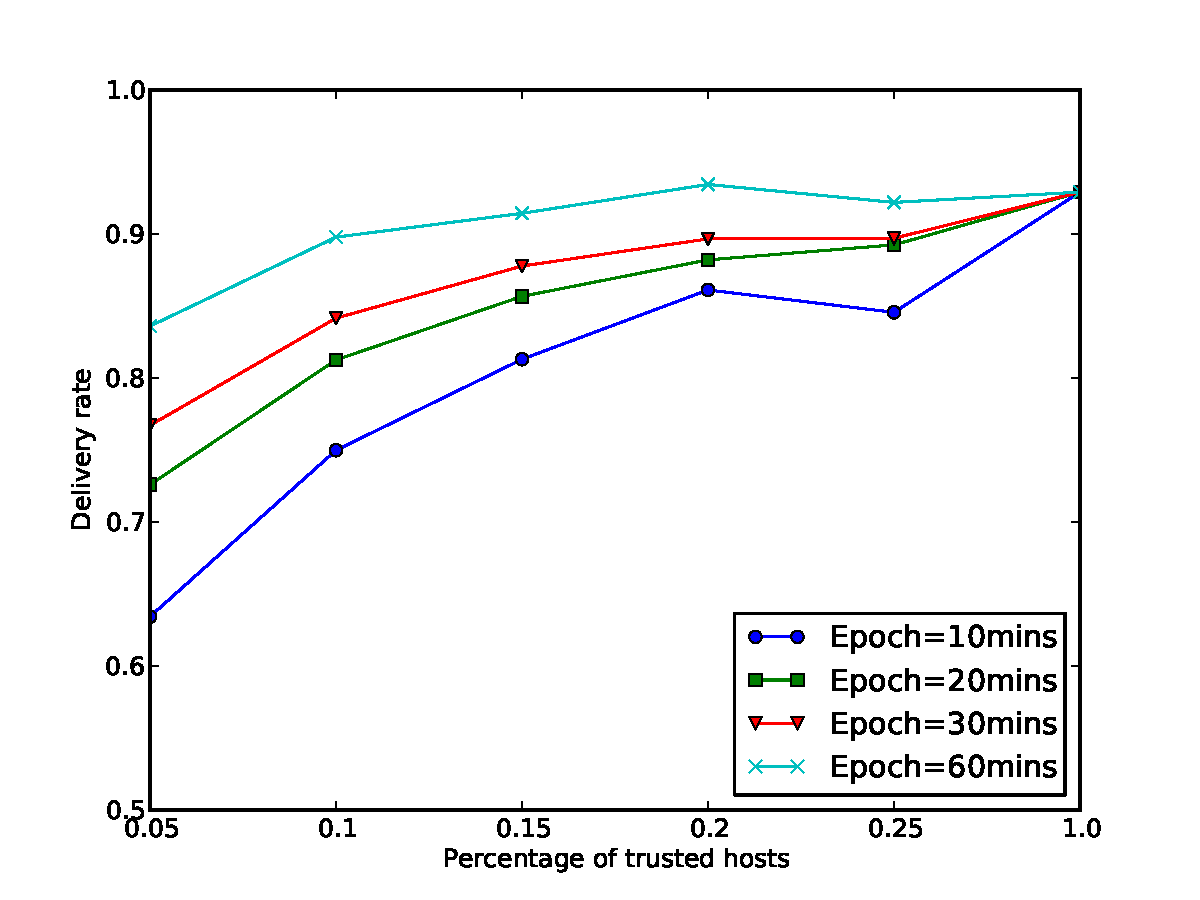
\includegraphics[width=0.33\columnwidth]{figures/epoch_3/delivery_rate.pdf}
\label{fig:delivery_rate_3}
}
%\hfill
\subfloat[Ephemeral ID valid for 6 epochs]{%
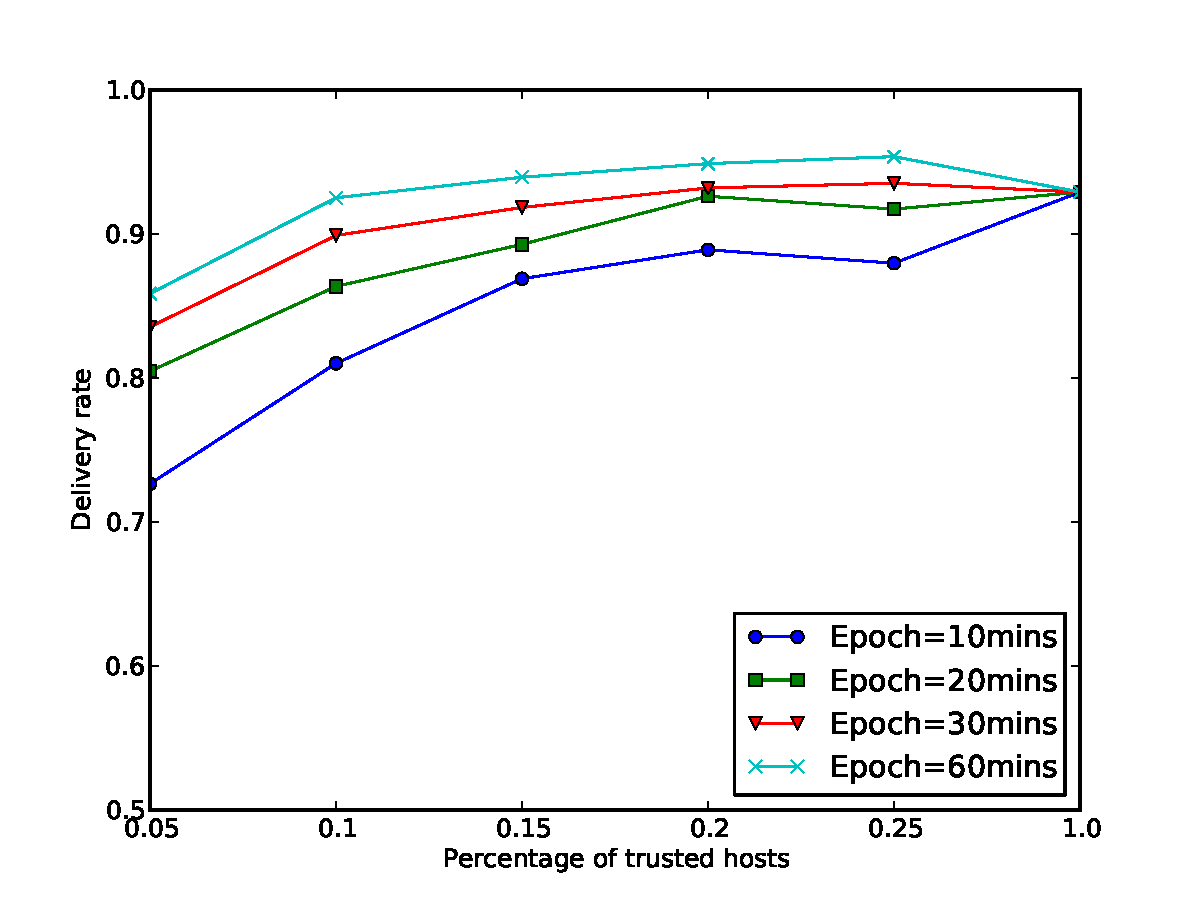
\includegraphics[width=0.33\columnwidth]{figures/epoch_6/delivery_rate.pdf}
\label{fig:delivery_rate_6}
}
%\hfill
\subfloat[Ephemeral ID valid for 6 epochs. Infinite packet buffer.]{%
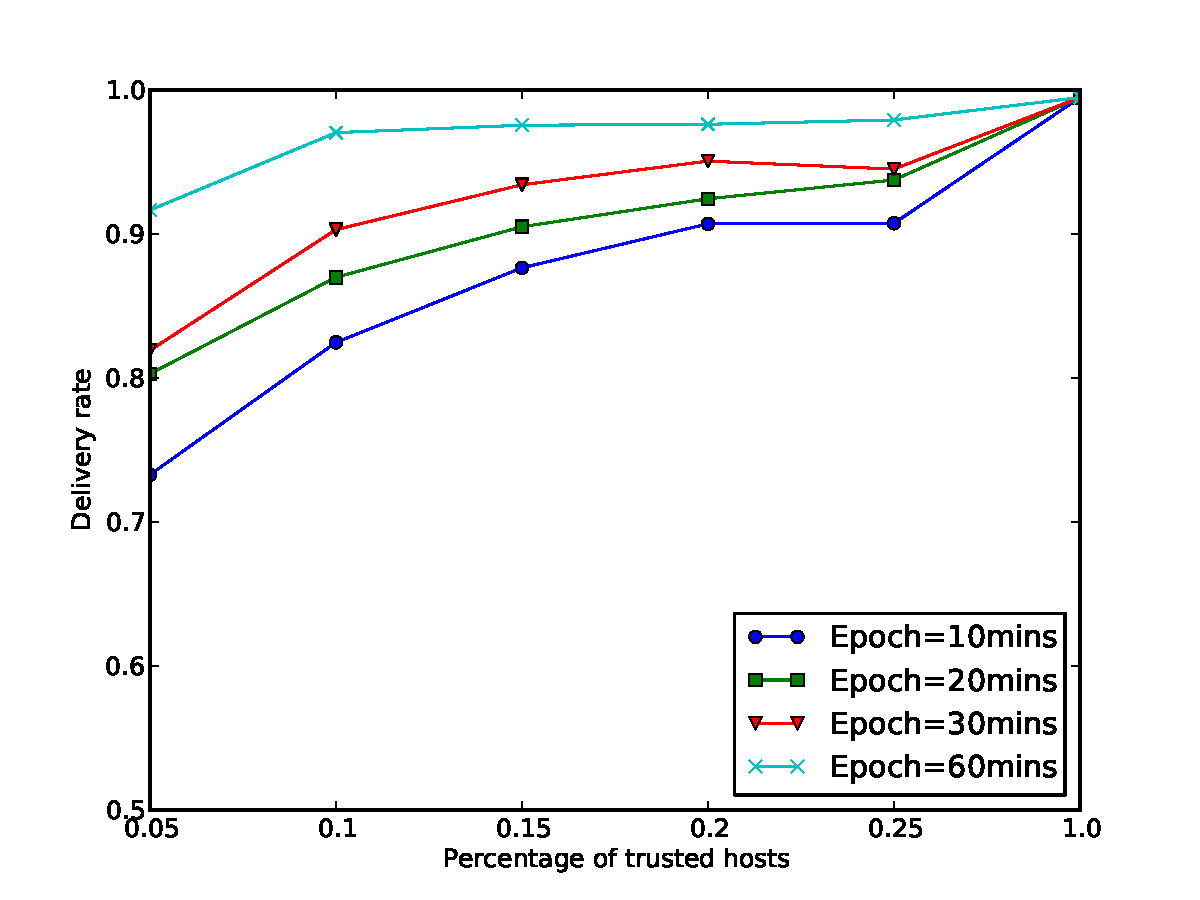
\includegraphics[width=0.33\columnwidth]{figures/epoch_6_maxbuffer/delivery_rate.pdf}
\label{fig:delivery_rate_6_maxbuffer}
}
\caption{{\bf Packet delivery rate.} 
Delivery rate of pure epidemic routing: 92.91\%.  
Delivery rate of pure epidemic routing with infinite packet buffer: 99.48\%.
Increasing ephemeral ID duration from 3 epochs to 6 epochs enhances the delivery rate significantly. 
In Figure~\ref{fig:delivery_rate_6_maxbuffer}, ephemeral ID expiry does not occur when epoch is 60 mins. 
[TTL (5 hours) $<$ Epoch (1 hour) * Ephemeral ID duration (6 epochs)]
In this case, packet drop occurs only when TTL expires, and the delivery rate is almost as high as that of epidemic (flooding) routing 
}
\label{fig:delivery_rate}
\end{figure}


% delivery latency
\begin{figure}[h!]
\center
\subfloat[Ephemeral ID valid for 3 epoch]{%
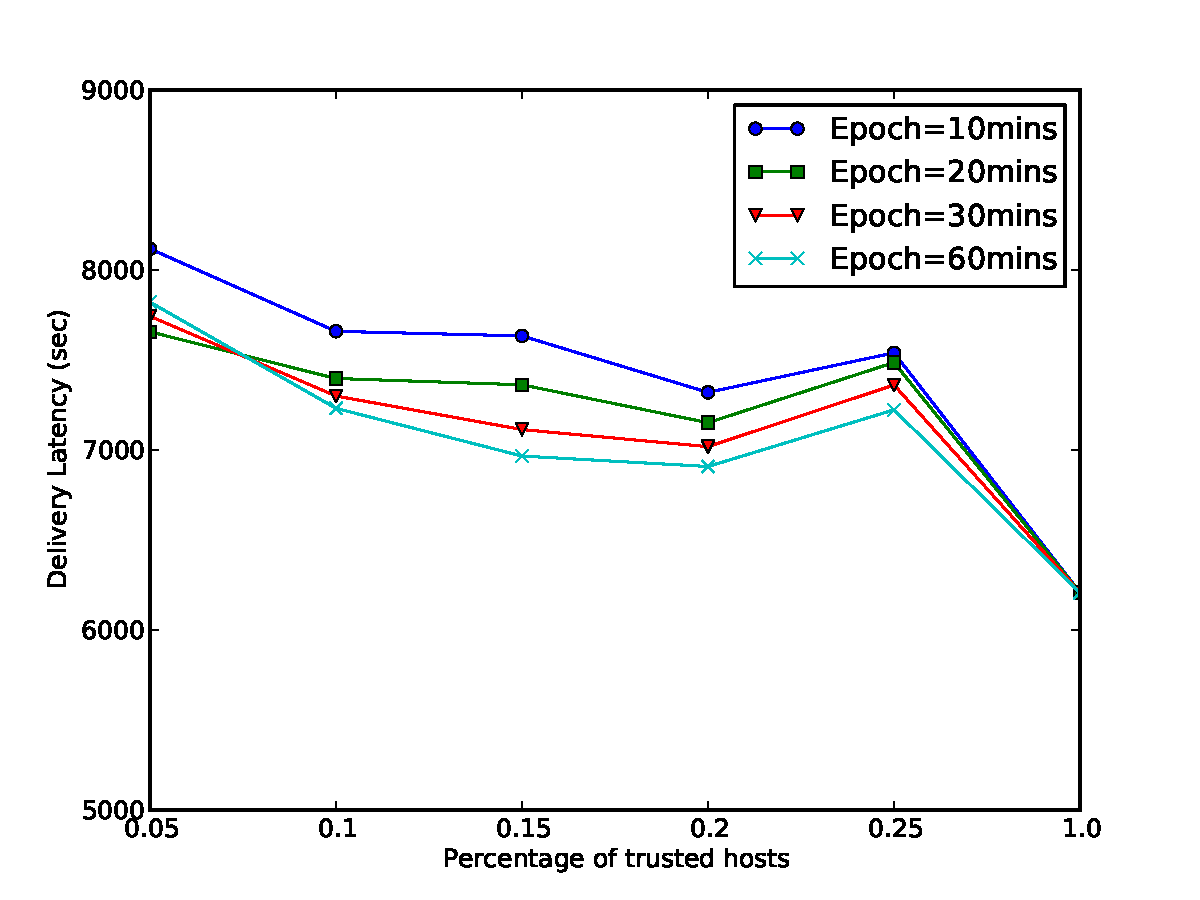
\includegraphics[width=0.33\columnwidth]{figures/epoch_3/delivery_latency.pdf}
\label{fig:delivery_latency_3}
}
%\hfill
\subfloat[Ephemeral ID valid for 6 epochs]{%
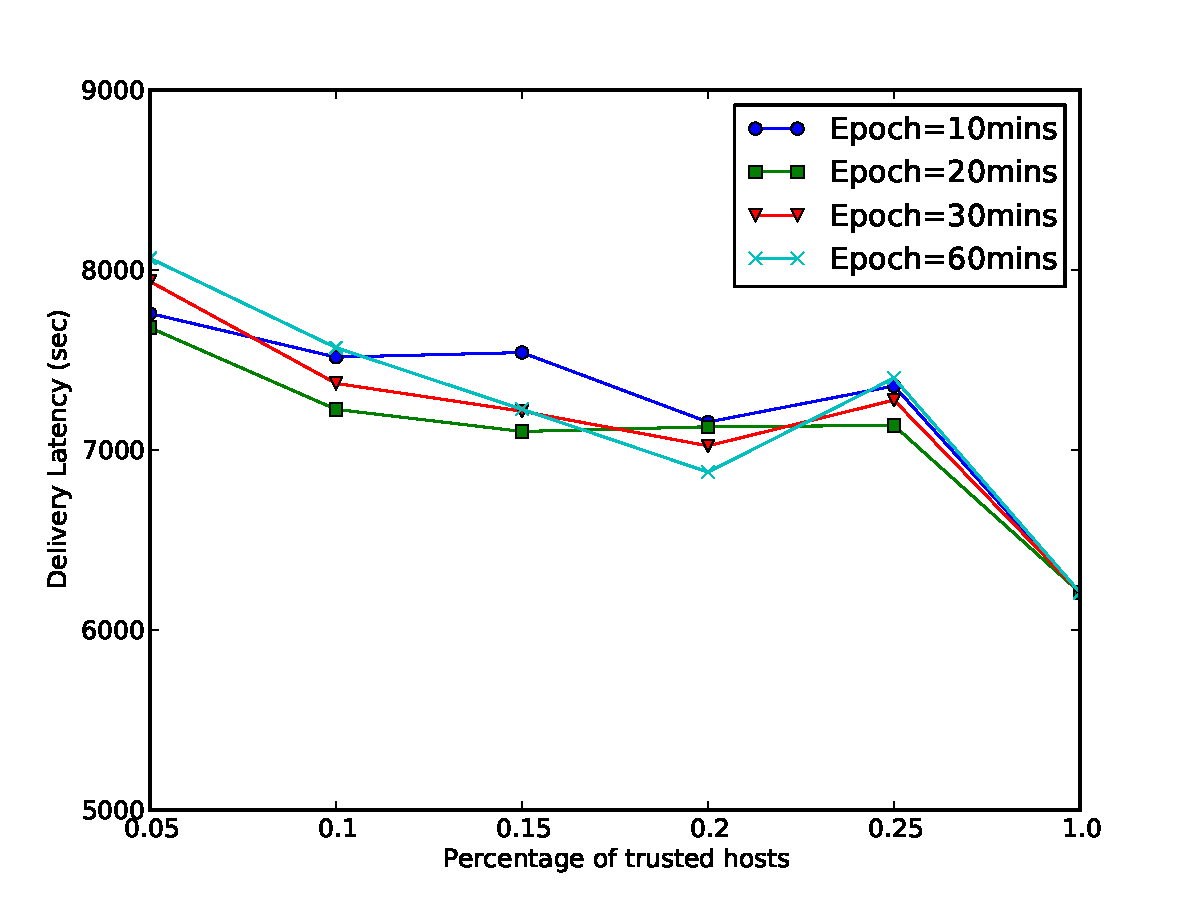
\includegraphics[width=0.33\columnwidth]{figures/epoch_6/delivery_latency.pdf}
\label{fig:delivery_latency_6}
}
%\hfill
\subfloat[Ephemeral ID valid for 6 epochs. Infinite packet buffer.]{%
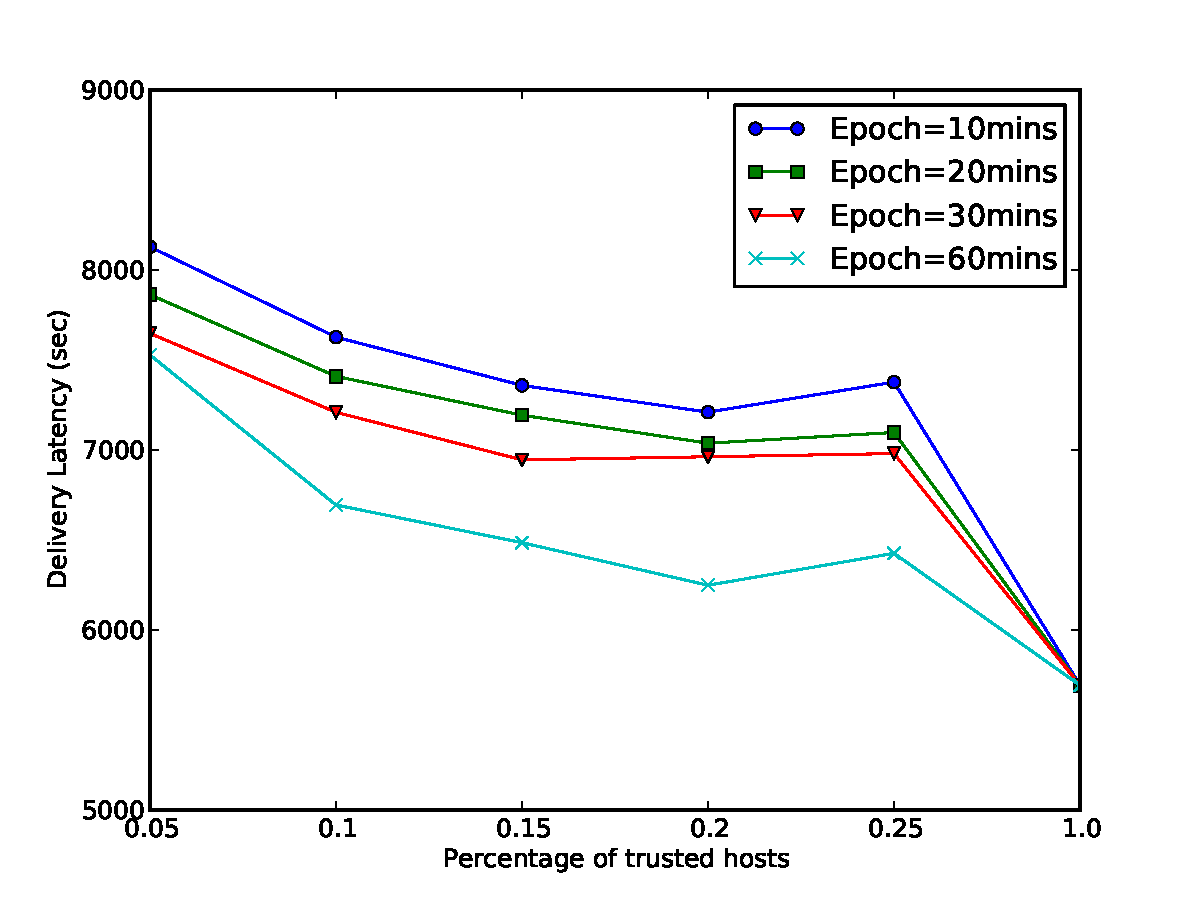
\includegraphics[width=0.33\columnwidth]{figures/epoch_6_maxbuffer/delivery_latency.pdf}
\label{fig:delivery_latency_6}
}

\caption{{\bf Packet delivery latency.}
With finite packet buffer, delivery latency of our protocol is 1000 - 2000 secs longer than that of flooding protocol.
}
\label{fig:delivery_latency}
\end{figure}




% hop count
\begin{figure}[h!]
\center
\subfloat[Ephemeral ID valid for 3 epochs]{%
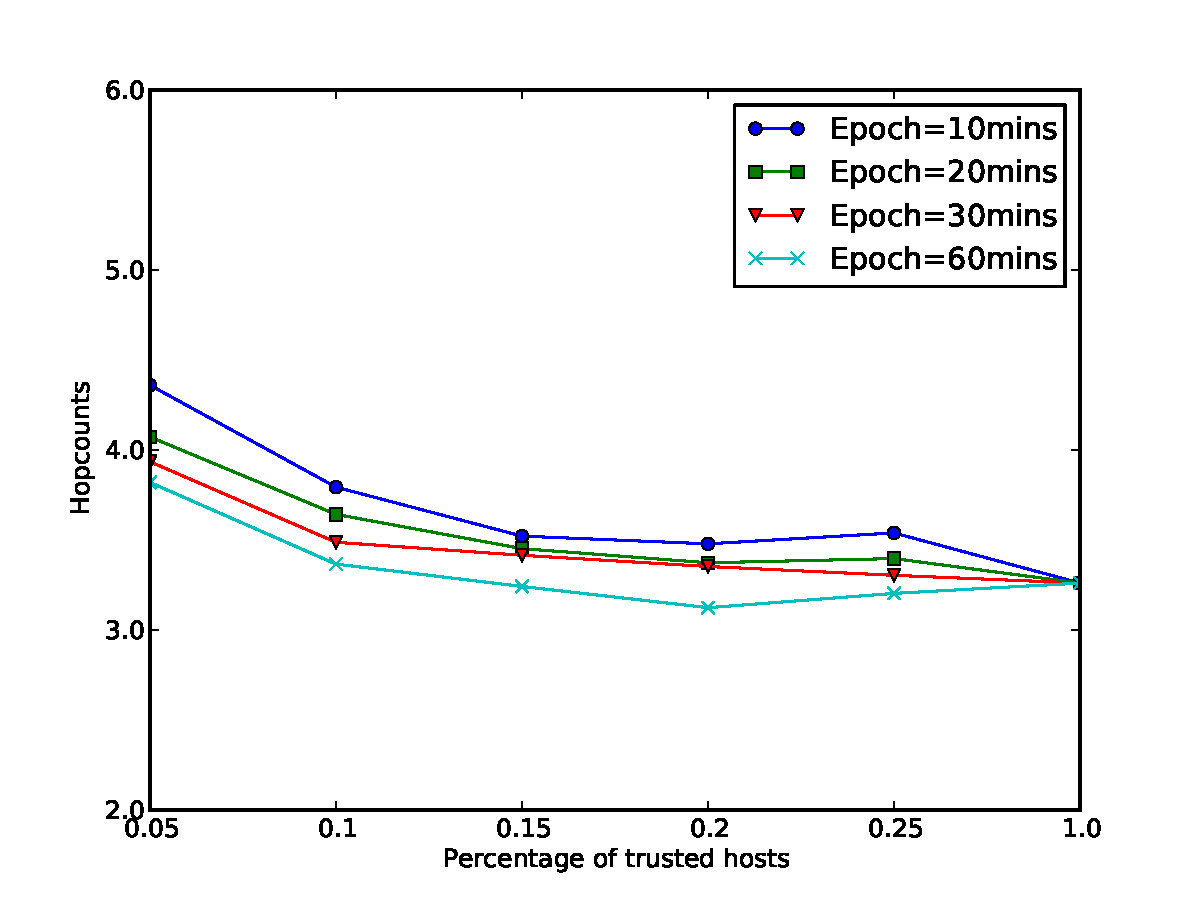
\includegraphics[width=0.33\columnwidth]{figures/epoch_3/hopcount.pdf}
\label{fig:delivery_hopcount_3}
}
%\hfill
\subfloat[Ephemeral ID valid for 6 epochs]{%
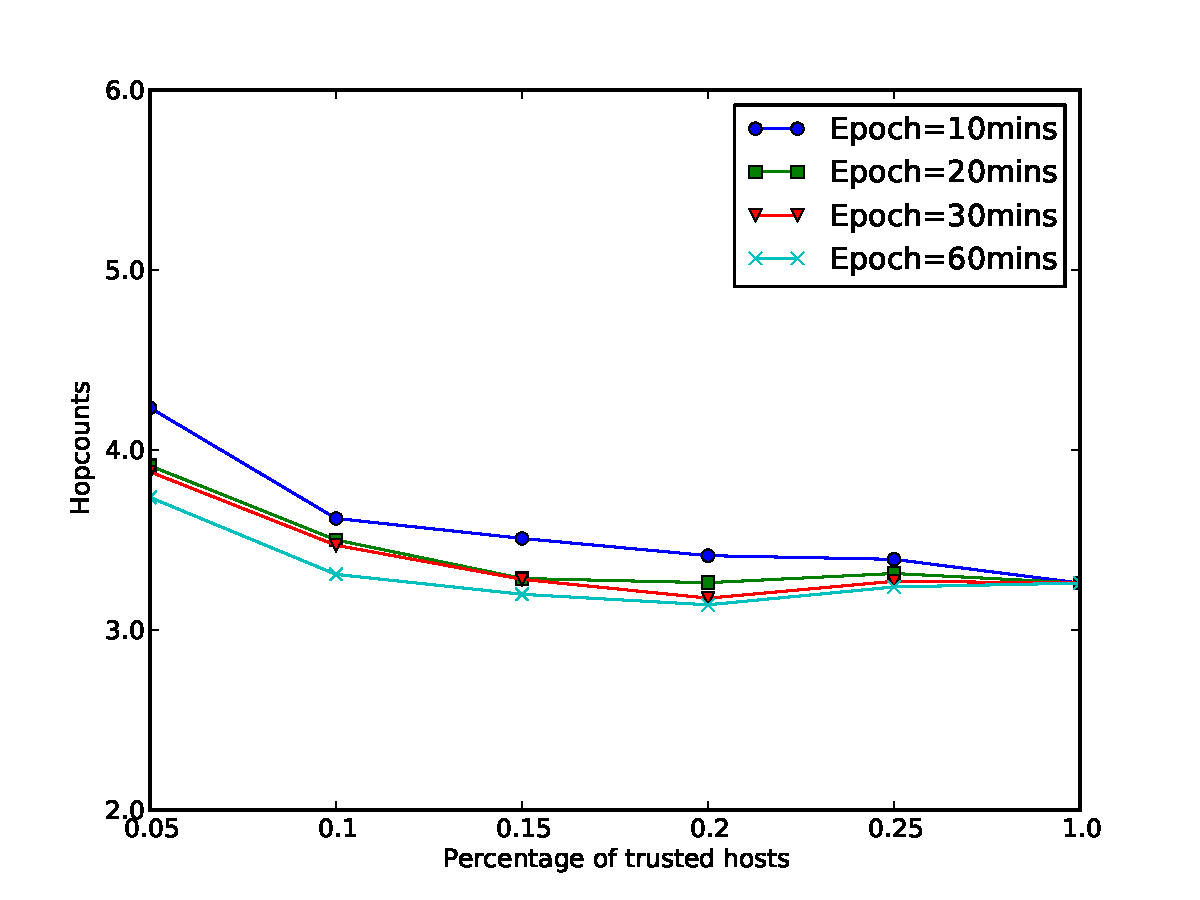
\includegraphics[width=0.33\columnwidth]{figures/epoch_6/hopcount.pdf}
\label{fig:delivery_hopcount_6}
}
%\hfill
\subfloat[Ephemeral ID valid for 6 epochs. Infinite packet buffer.]{%
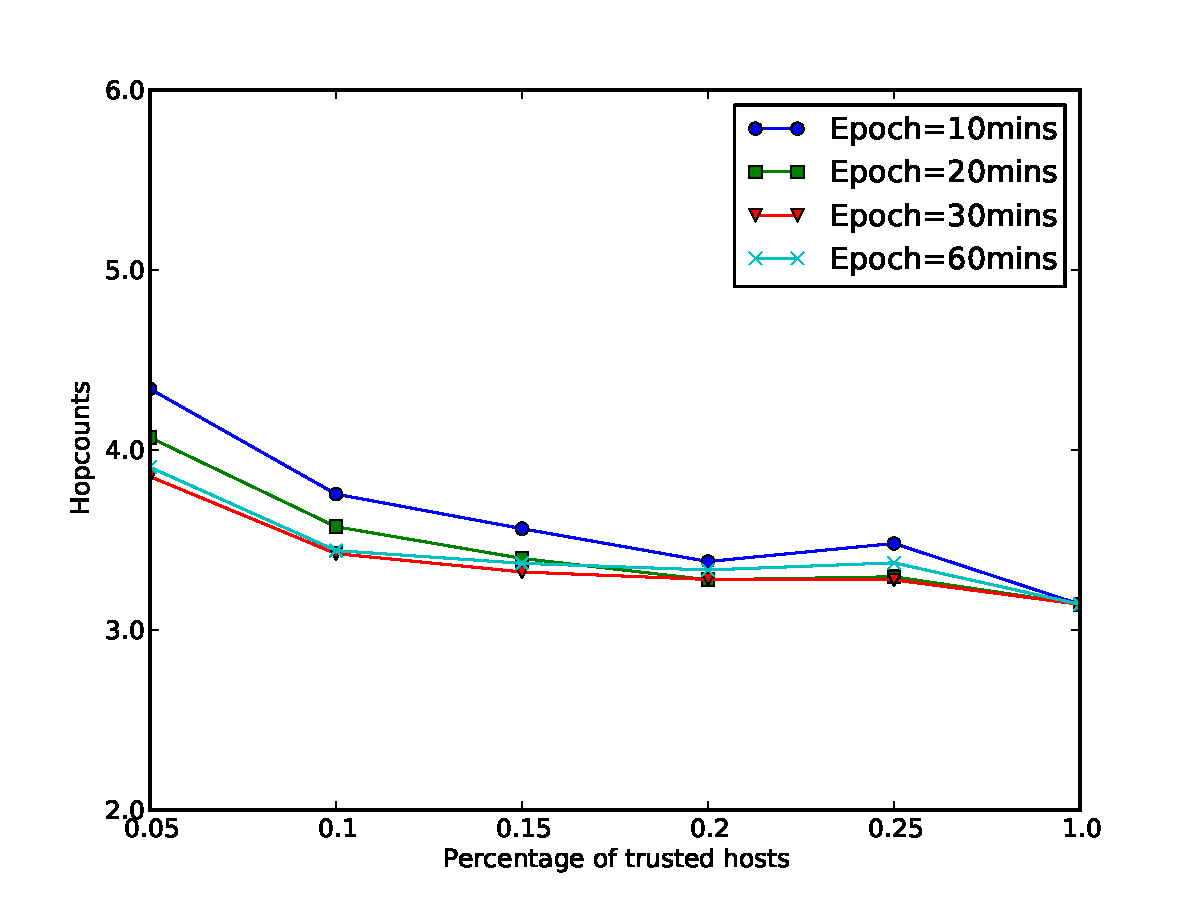
\includegraphics[width=0.33\columnwidth]{figures/epoch_6_maxbuffer/hopcount.pdf}
\label{fig:delivery_hopcount_6}
}
\caption{{\bf Packet delivery hop count.}
In general, delivery hop count is increased by less than 1 hop. 
}
\label{fig:delivery_hopcount}
\end{figure}








% overall packet relay count / delivered packet relay count 
\begin{figure}[h!]
\center
\subfloat[Overall packets. Ephemeral ID valid for 3 epochs.]{%
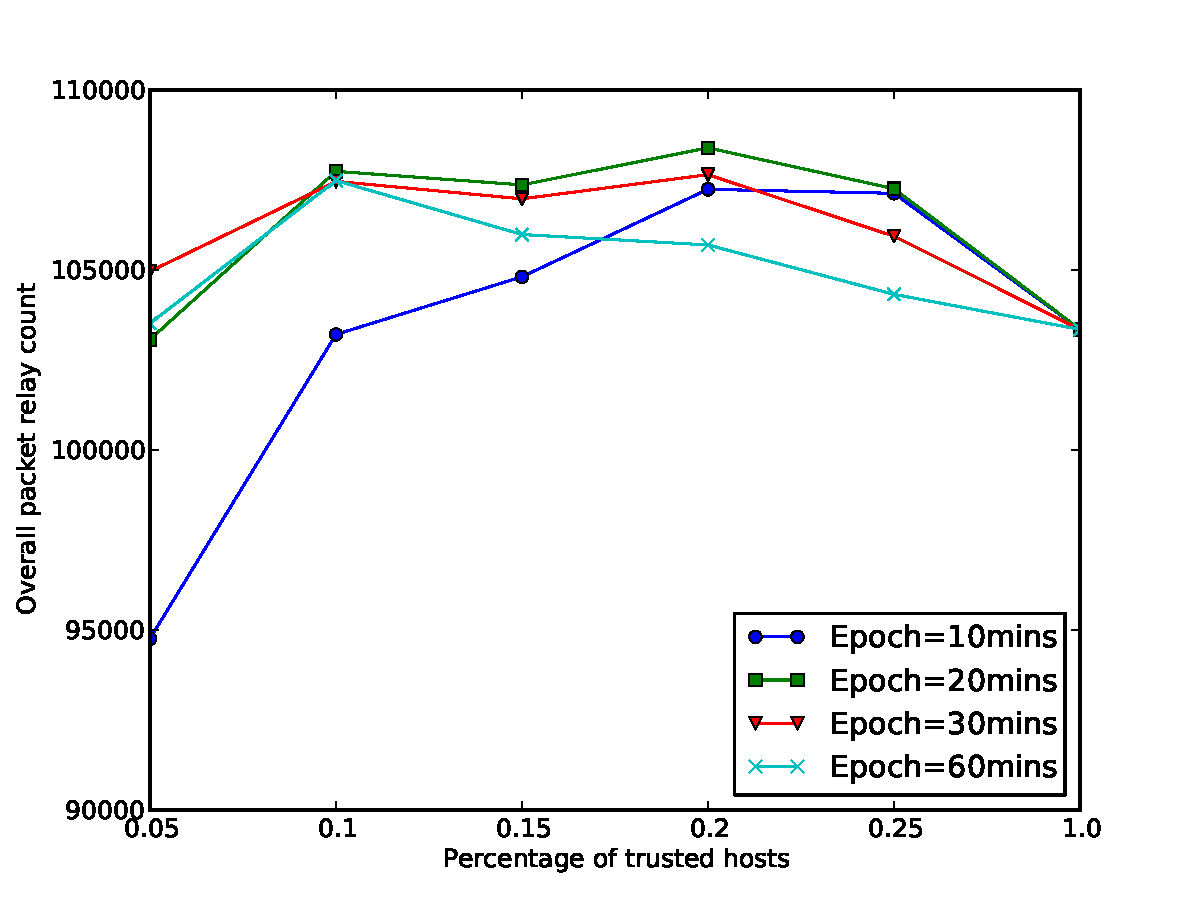
\includegraphics[width=0.33\columnwidth]{figures/epoch_3/relay_count.pdf}
\label{fig:relay_count_epoch_3}
}
%\hfill
\subfloat[Overall packets. Ephemeral ID valid for 6 epochs.]{%
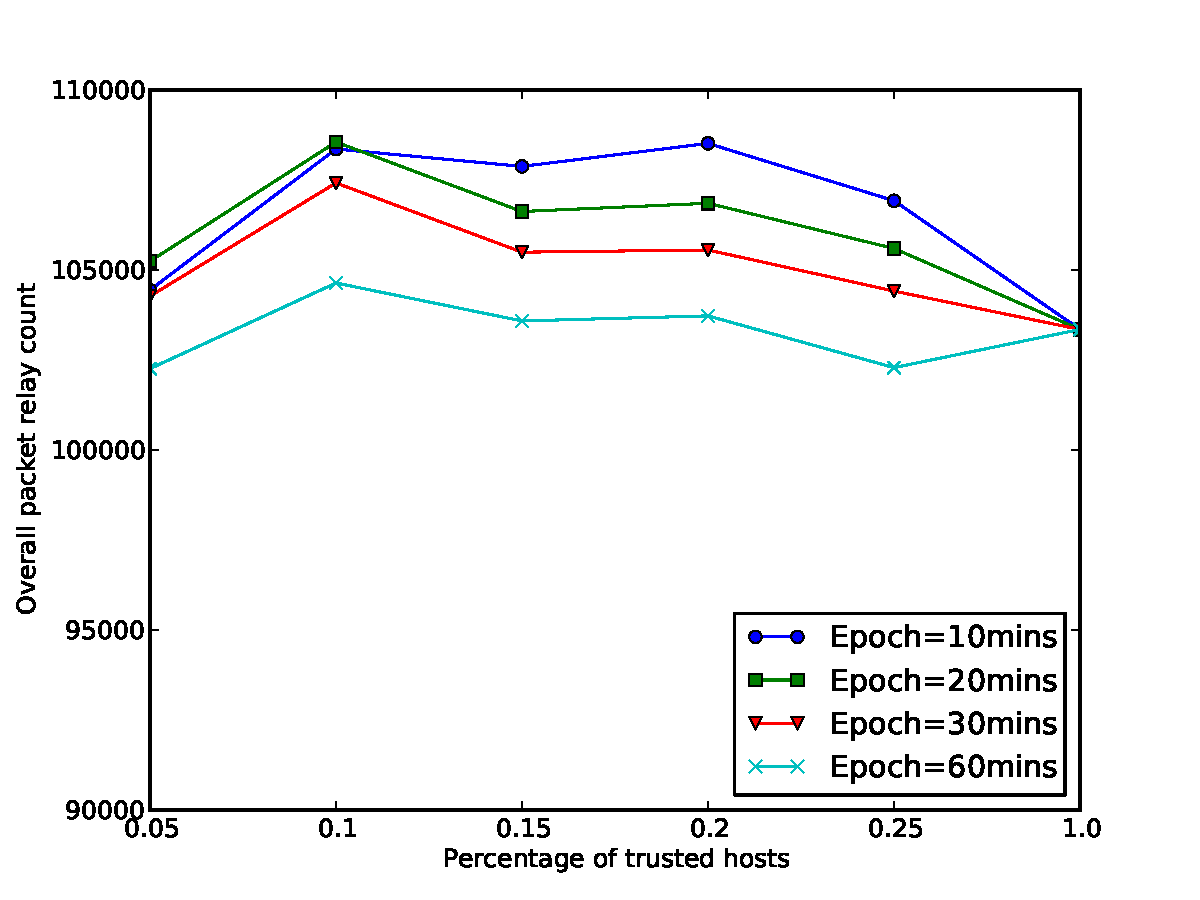
\includegraphics[width=0.33\columnwidth]{figures/epoch_6/relay_count.pdf}
\label{fig:relay_count_epoch_6}
}
%\hfill
\subfloat[Overall packets. Ephemeral ID valid for 6 epochs. Infinite packet buffer.]{%
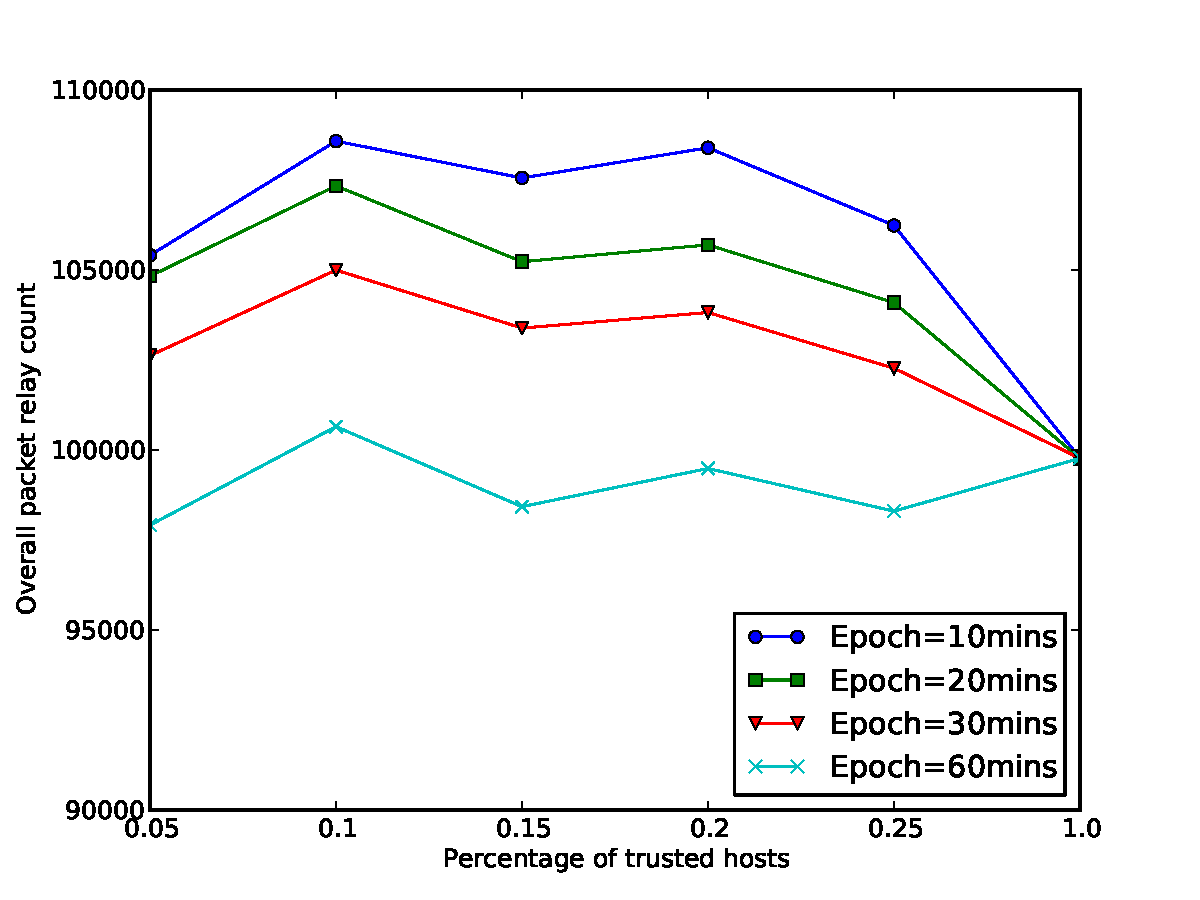
\includegraphics[width=0.33\columnwidth]{figures/epoch_6_maxbuffer/relay_count.pdf}
\label{fig:relay_count_epoch_6}
}
\hfill
\subfloat[Delivered packets. Ephemeral ID valid for 3 epochs.]{%
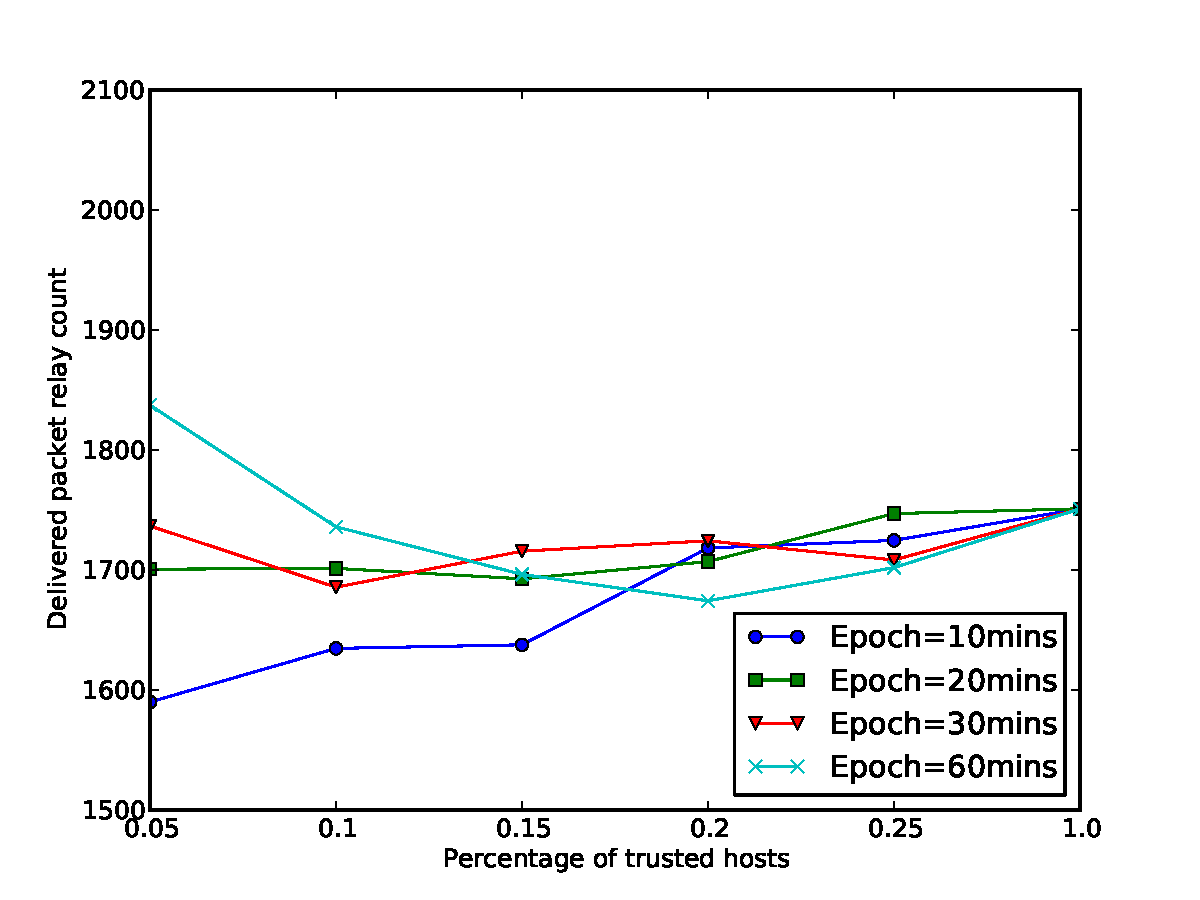
\includegraphics[width=0.33\columnwidth]{figures/epoch_3/relay_delivery_count.pdf}
\label{fig:relay_delivery_count_epoch_3}
}
%\hfill
\subfloat[Delivered packets. Ephemeral ID valid for 6 epochs.]{%
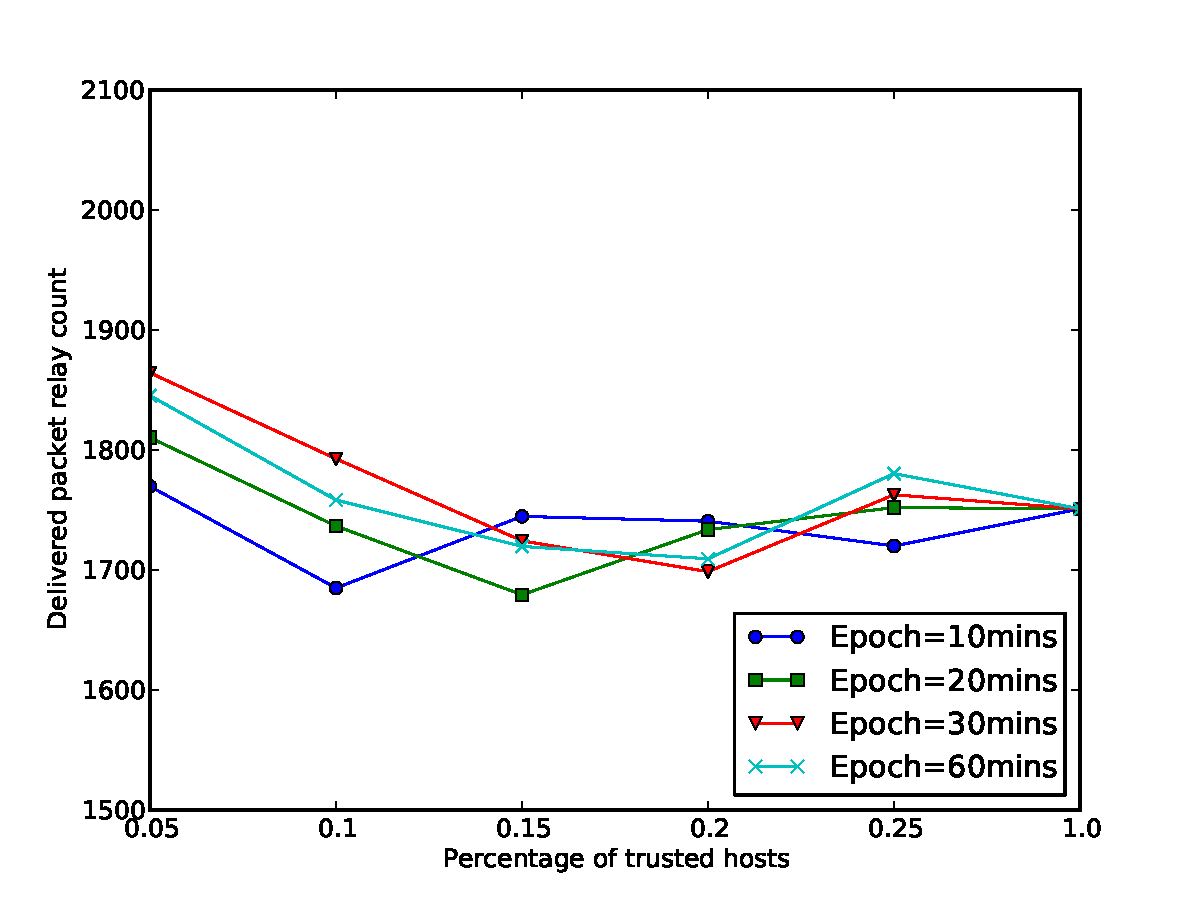
\includegraphics[width=0.33\columnwidth]{figures/epoch_6/relay_delivery_count.pdf}
\label{fig:relay_delivery_count_epoch_6}
}
\subfloat[Delivered packets. Ephemeral ID valid for 6 epochs. Infinite packet buffer.]{%
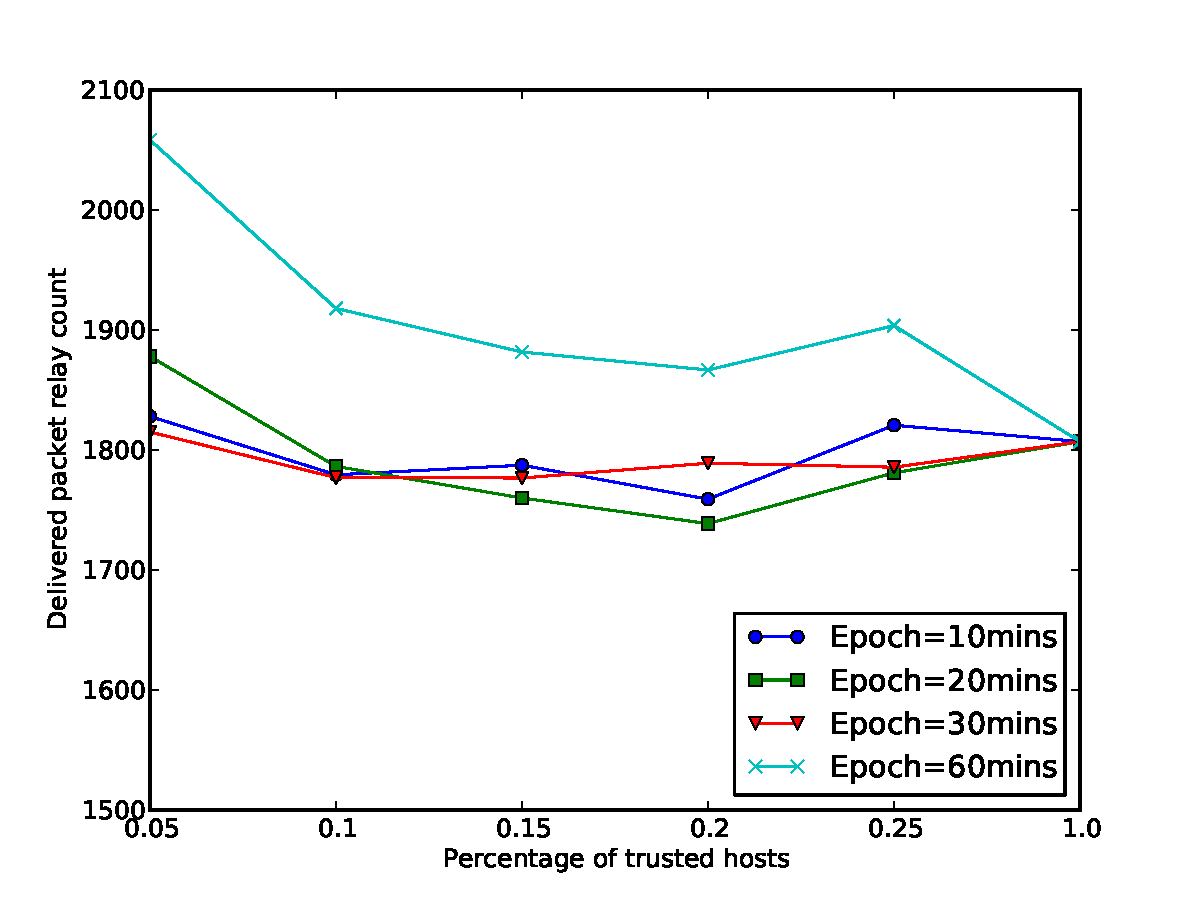
\includegraphics[width=0.33\columnwidth]{figures/epoch_6_maxbuffer/relay_delivery_count.pdf}
\label{fig:relay_delivery_count_epoch_6}
}

\caption{{\bf Packet relay count.}
Only about $2\%$ of packet relays are used for actual packet deliveries. 
}
\label{fig:relay_count}
\end{figure}







% packet relay classification over varying eppoch
\begin{figure}[h!]
\center
\subfloat[Overall packets. Ephemeral ID valid for 3 epochs]{%
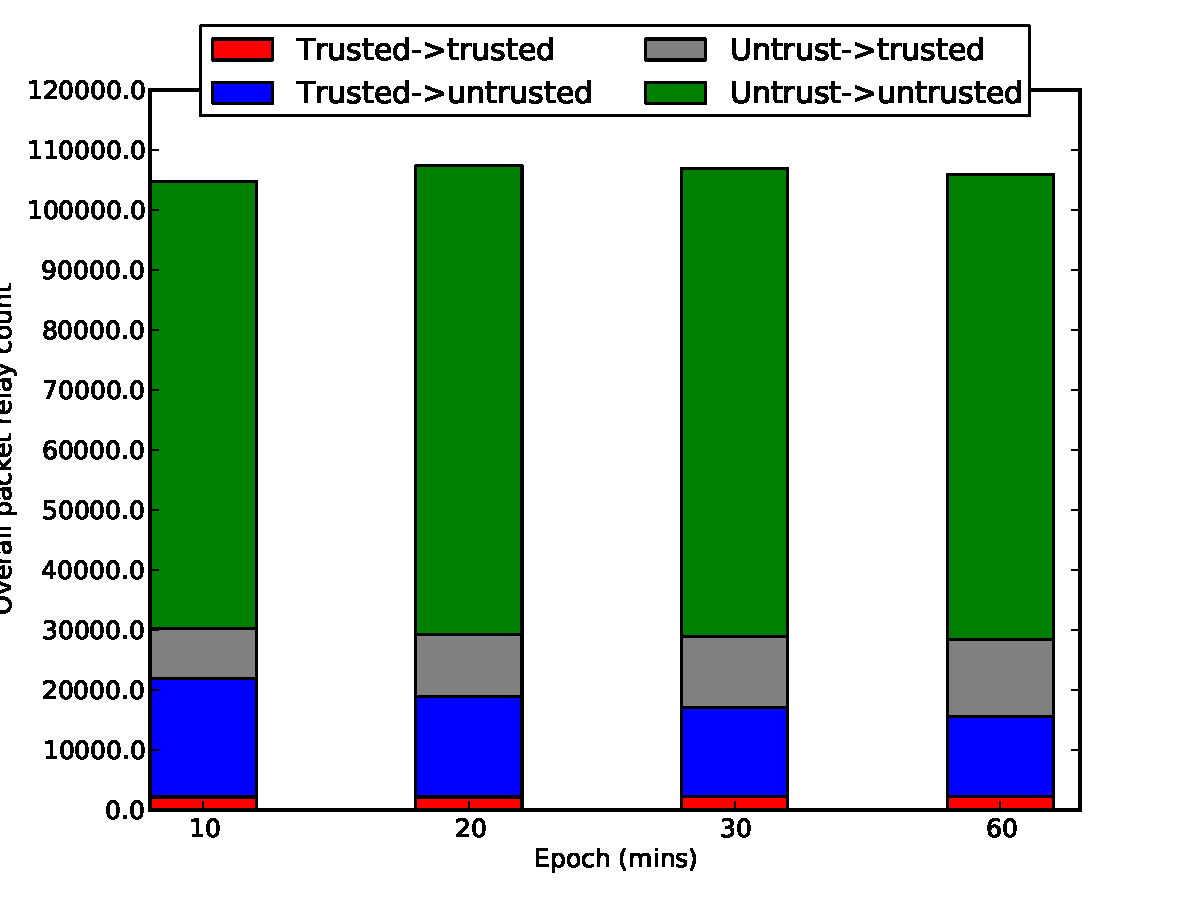
\includegraphics[width=0.33\columnwidth]{figures/epoch_3/relay_classification_over_epoch.pdf}
\label{fig:overall_relay_classification_epoch_3}
}
%\hfill
\subfloat[Overall packets. Ephemeral ID valid for 6 epochs]{%
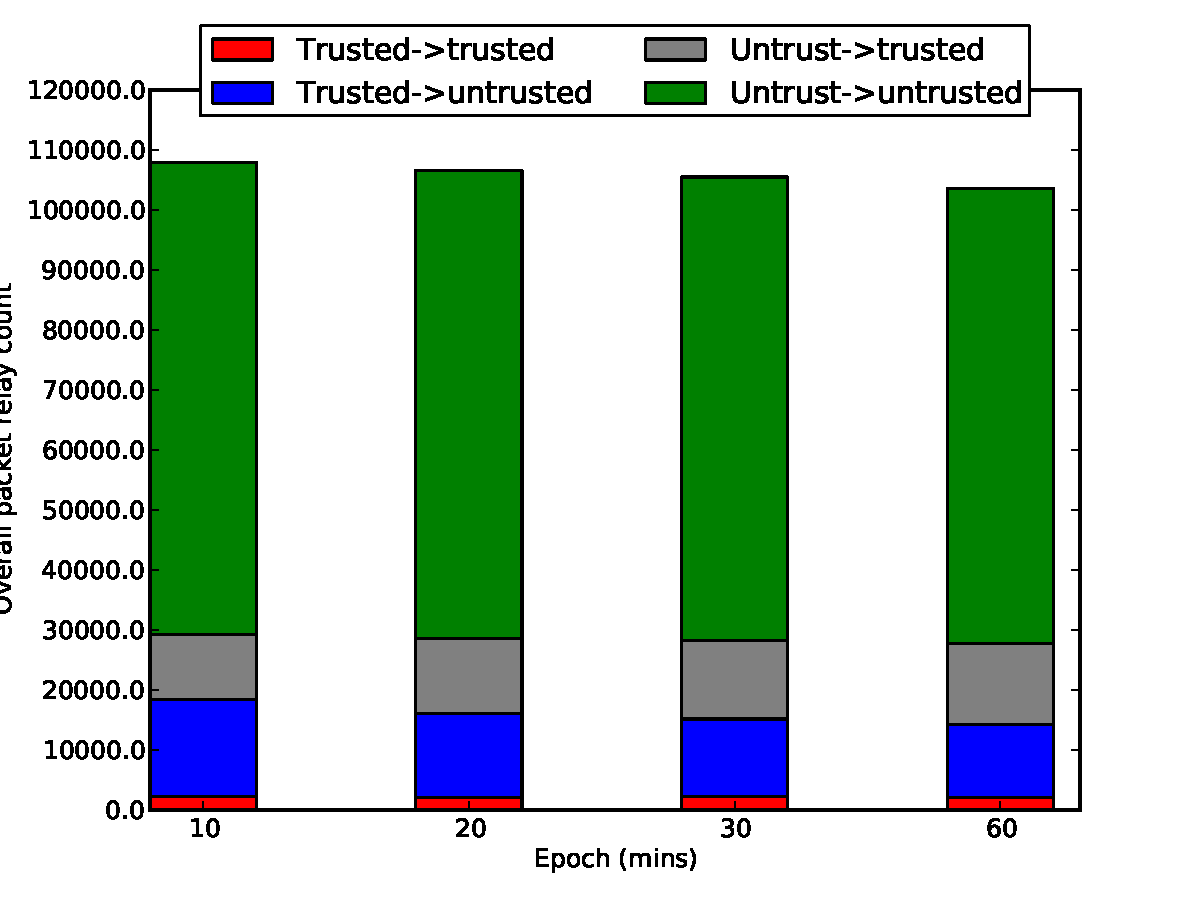
\includegraphics[width=0.33\columnwidth]{figures/epoch_6/relay_classification_over_epoch.pdf}
\label{fig:overall_relay_classification_epoch_6}
}
%\hfill
\subfloat[Overall packets. Ephemeral ID valid for 6 epochs. Infinite packet buffer.]{%
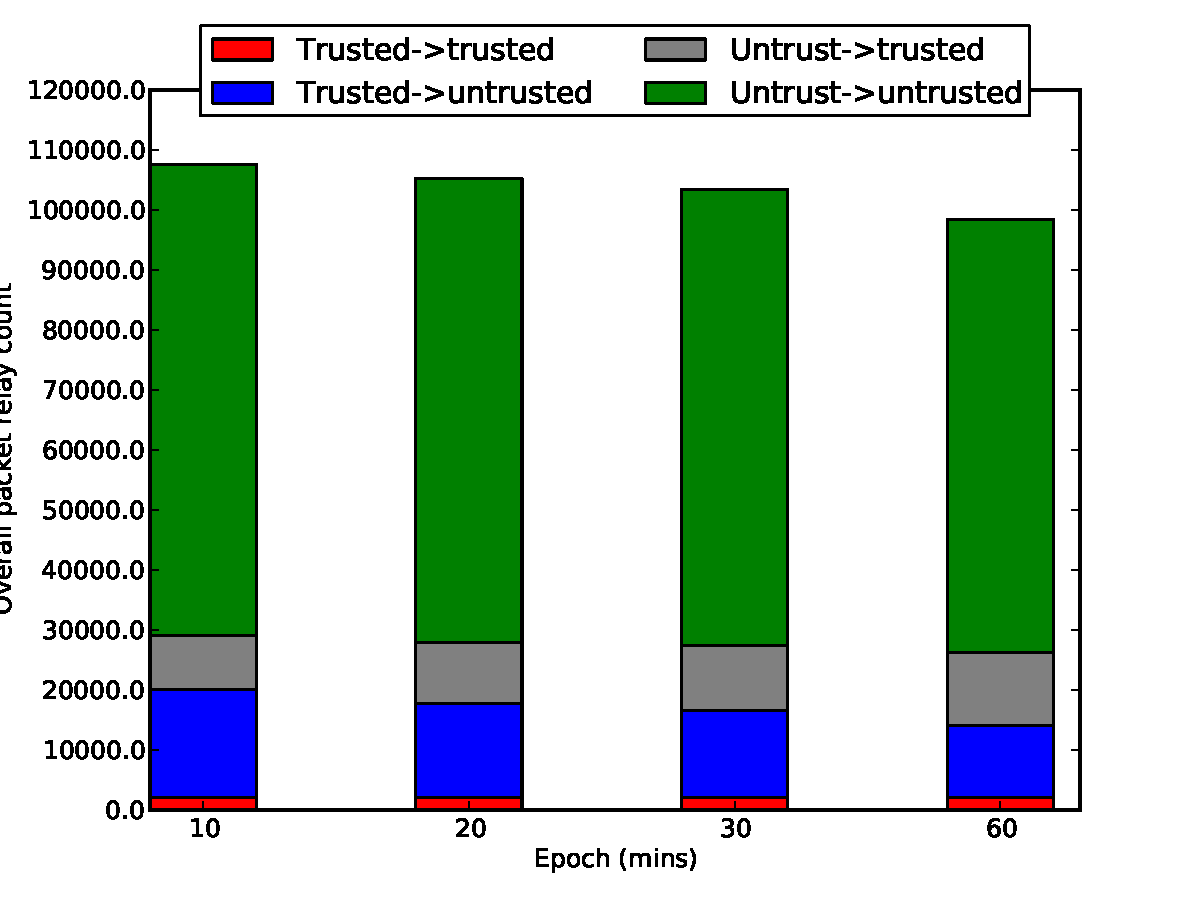
\includegraphics[width=0.33\columnwidth]{figures/epoch_6_maxbuffer/relay_classification_over_epoch.pdf}
\label{fig:overall_relay_classification_epoch_6}
}
\hfill
\subfloat[Delivered packets. Ephemeral ID valid for 3 epochs]{%
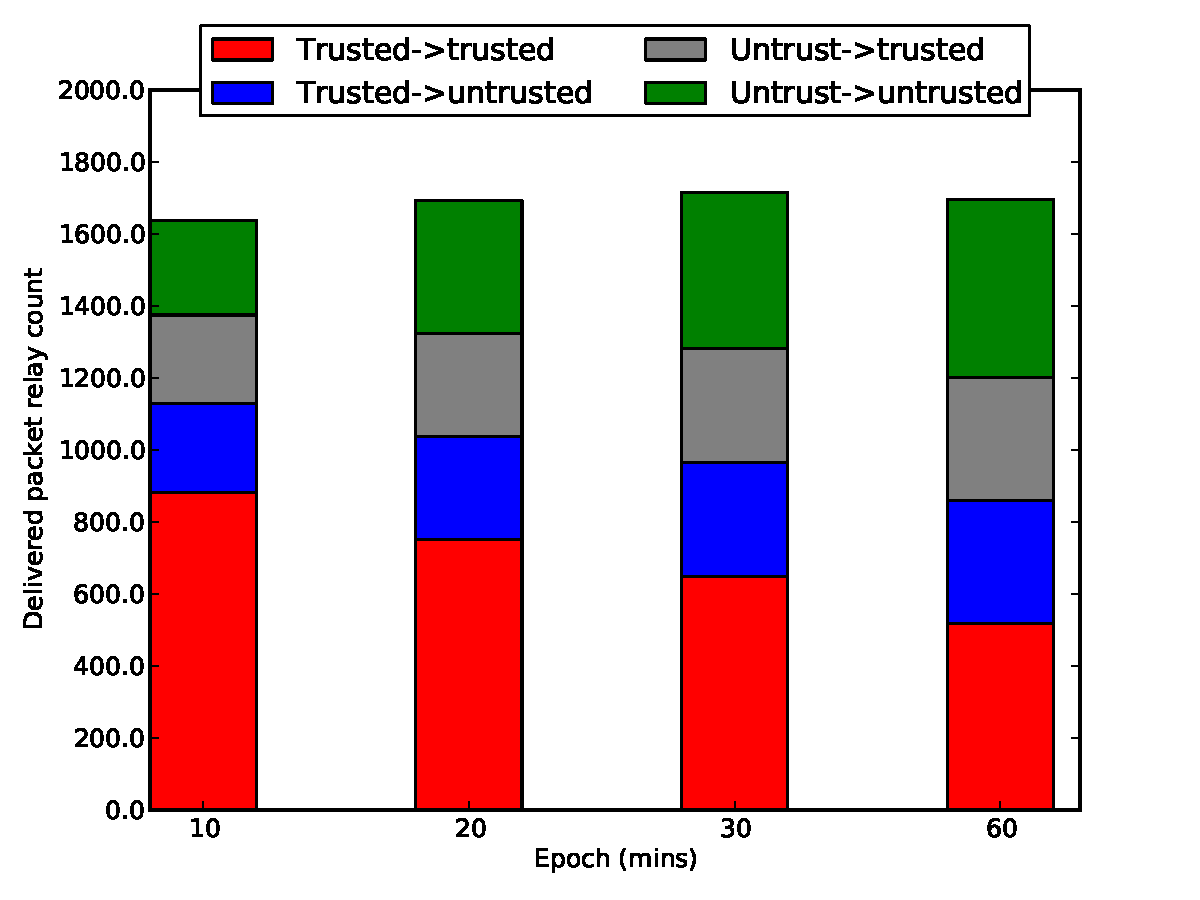
\includegraphics[width=0.33\columnwidth]{figures/epoch_3/relay_delivery_classification_over_epoch.pdf}
\label{fig:delivered_relay_classification_epoch_3}
}
%\hfill
\subfloat[Delivered packets. Ephemeral ID valid for 6 epochs]{%
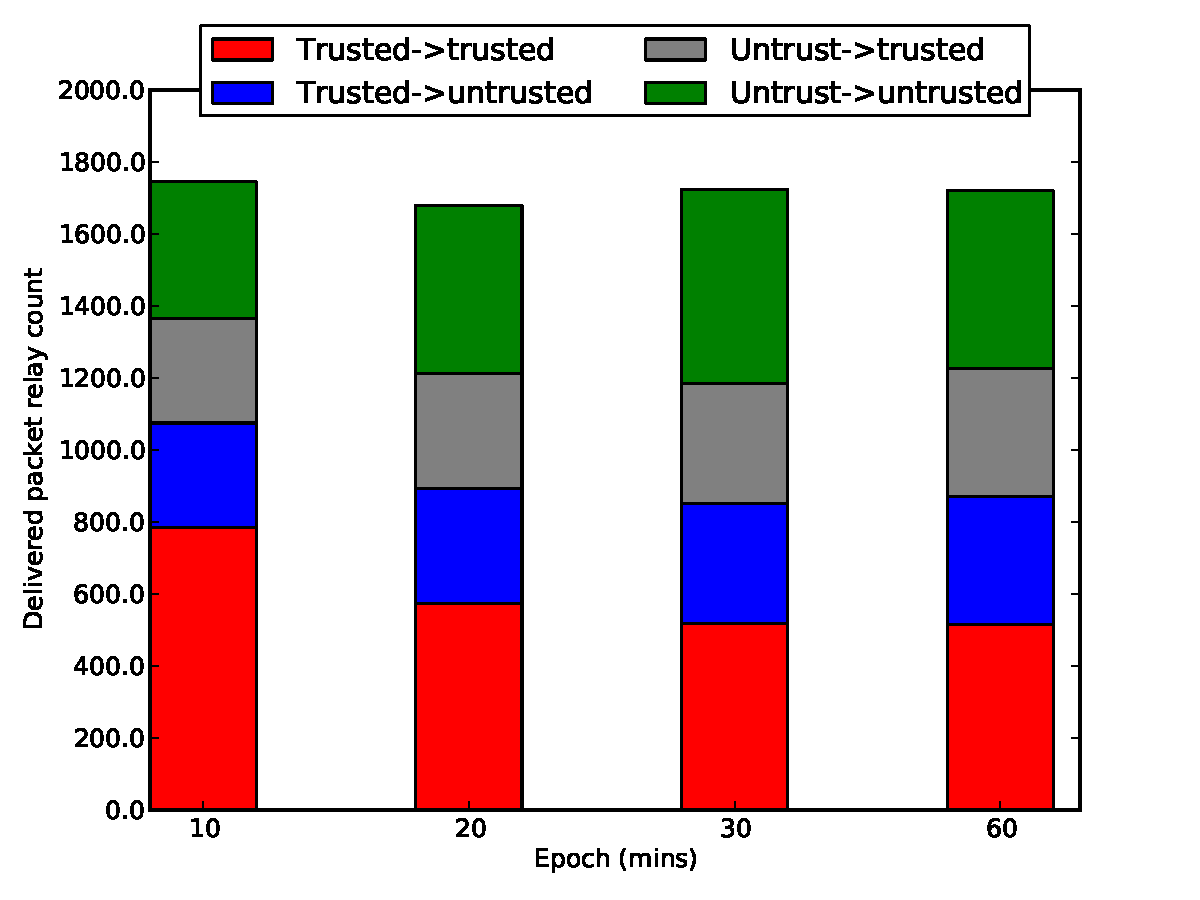
\includegraphics[width=0.33\columnwidth]{figures/epoch_6/relay_delivery_classification_over_epoch.pdf}
\label{fig:delivered_relay_classification_epoch_6}
}
%\hfill
\subfloat[Delivered packets. Ephemeral ID valid for 6 epochs. Infinite packet buffer]{%
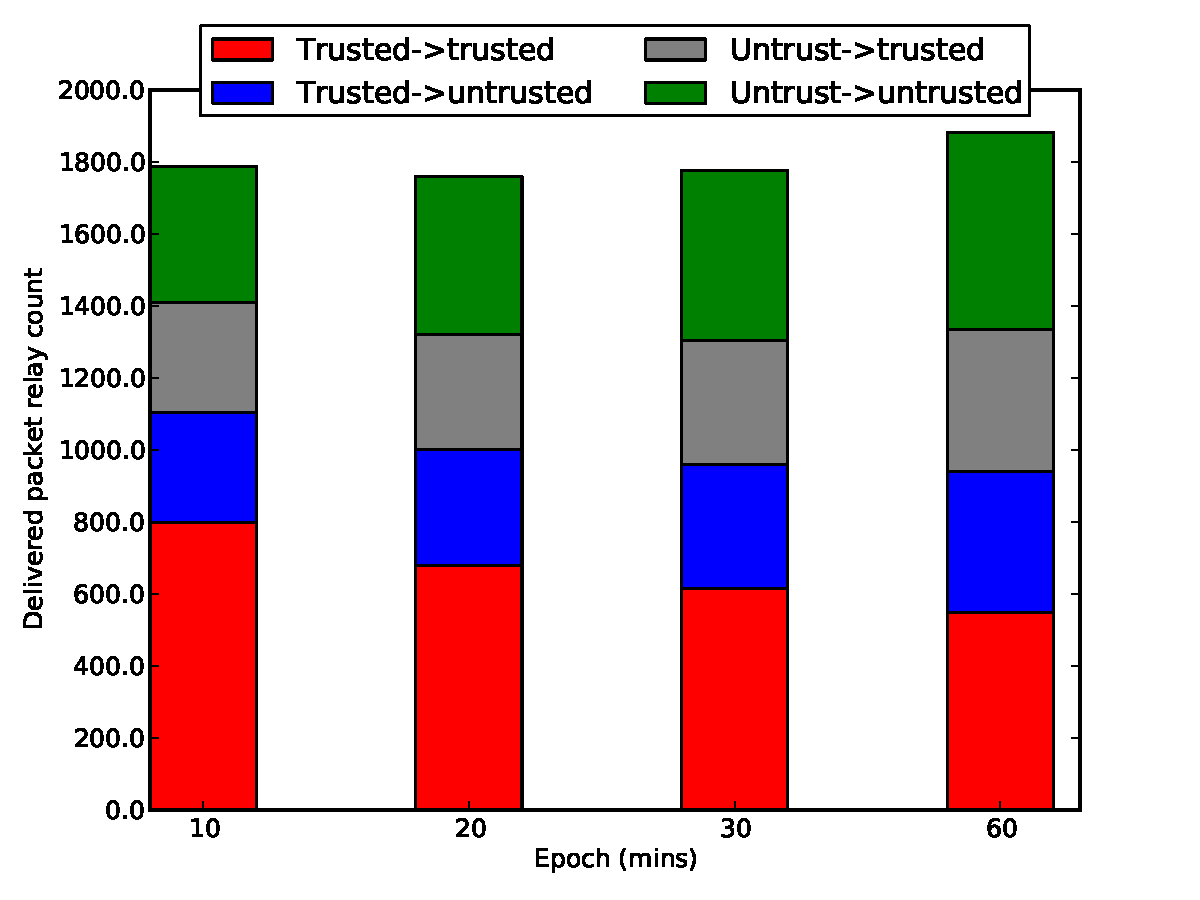
\includegraphics[width=0.33\columnwidth]{figures/epoch_6_maxbuffer/relay_delivery_classification_over_epoch.pdf}
\label{fig:delivered_relay_classification_epoch_6_maxbuffer}
}

\caption{{\bf Packet relay classification over varying epoch. Percentage of trusted nodes is $15\%$.}
Ephemeral ID duration does not affect overall packet relay classification, but it affects delivered packet relay classification.  
When ephemeral ID duration is 6 epochs, packet relays between two trusted nodes are slightly decreased while other types of relays are increased. 
}
\label{fig:relay_classification_epoch}
\end{figure}







% packet relay classification over varying percentage of trusted nodes
\begin{figure}[h!]
\center
\subfloat[Overall packets. Ephemeral ID valid for 3 epochs.]{%
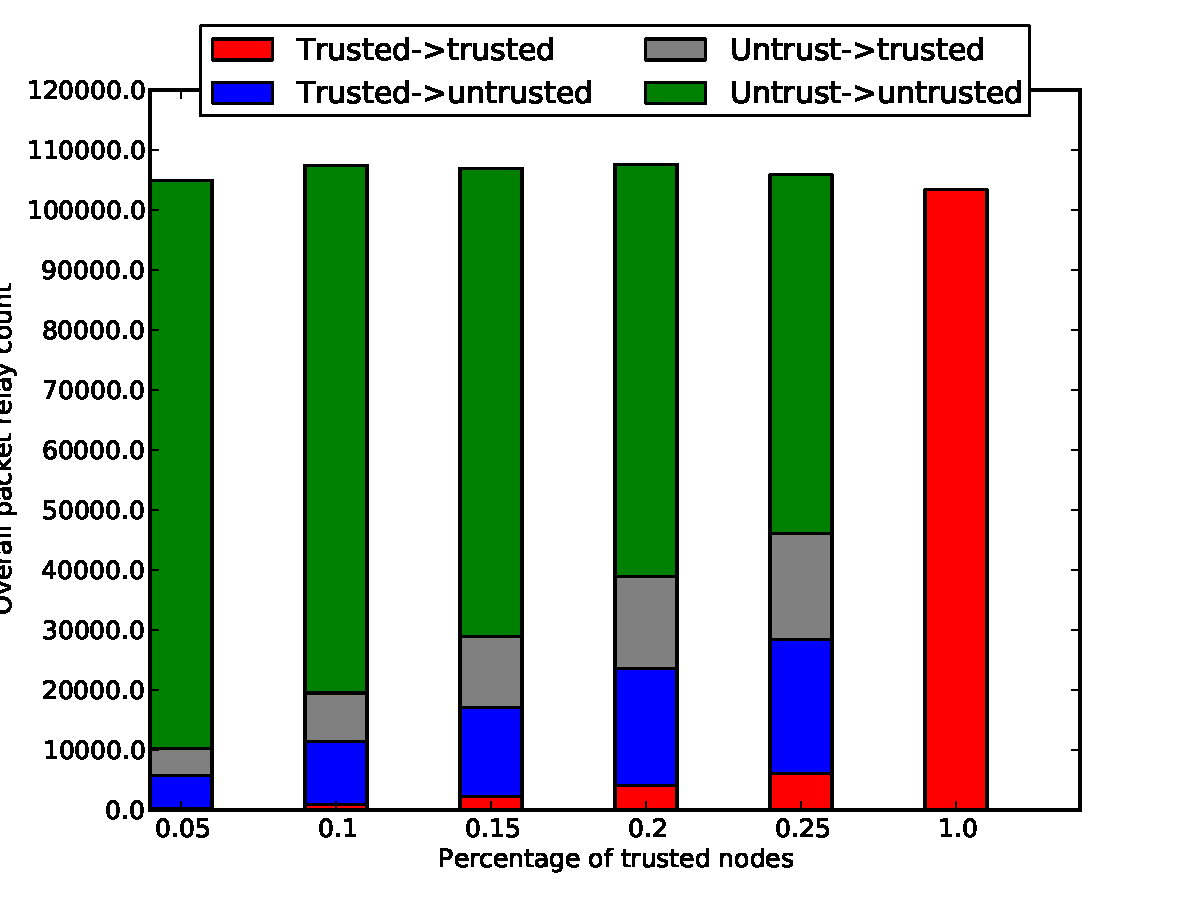
\includegraphics[width=0.33\columnwidth]{figures/epoch_3/relay_classification_over_percentage.pdf}
\label{fig:relay_classification_percentage_3}
}
%\hfill
\subfloat[Overall packets. Ephemeral ID valid for 6 epochs.]{%
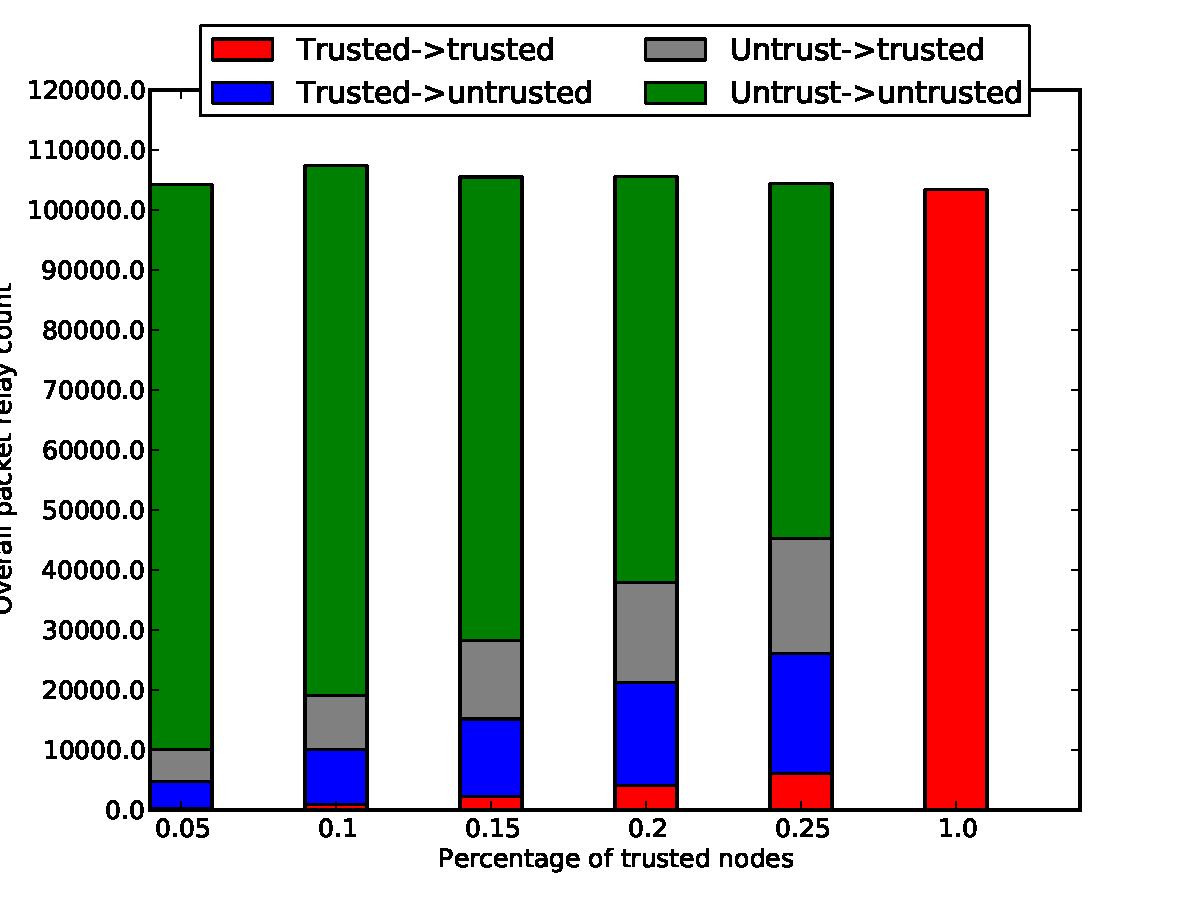
\includegraphics[width=0.33\columnwidth]{figures/epoch_6/relay_classification_over_percentage.pdf}
\label{fig:relay_classification_percentage_6}
}
%\hfill
\subfloat[Overall packets. Ephemeral ID valid for 6 epochs. Infinite packet buffer.]{%
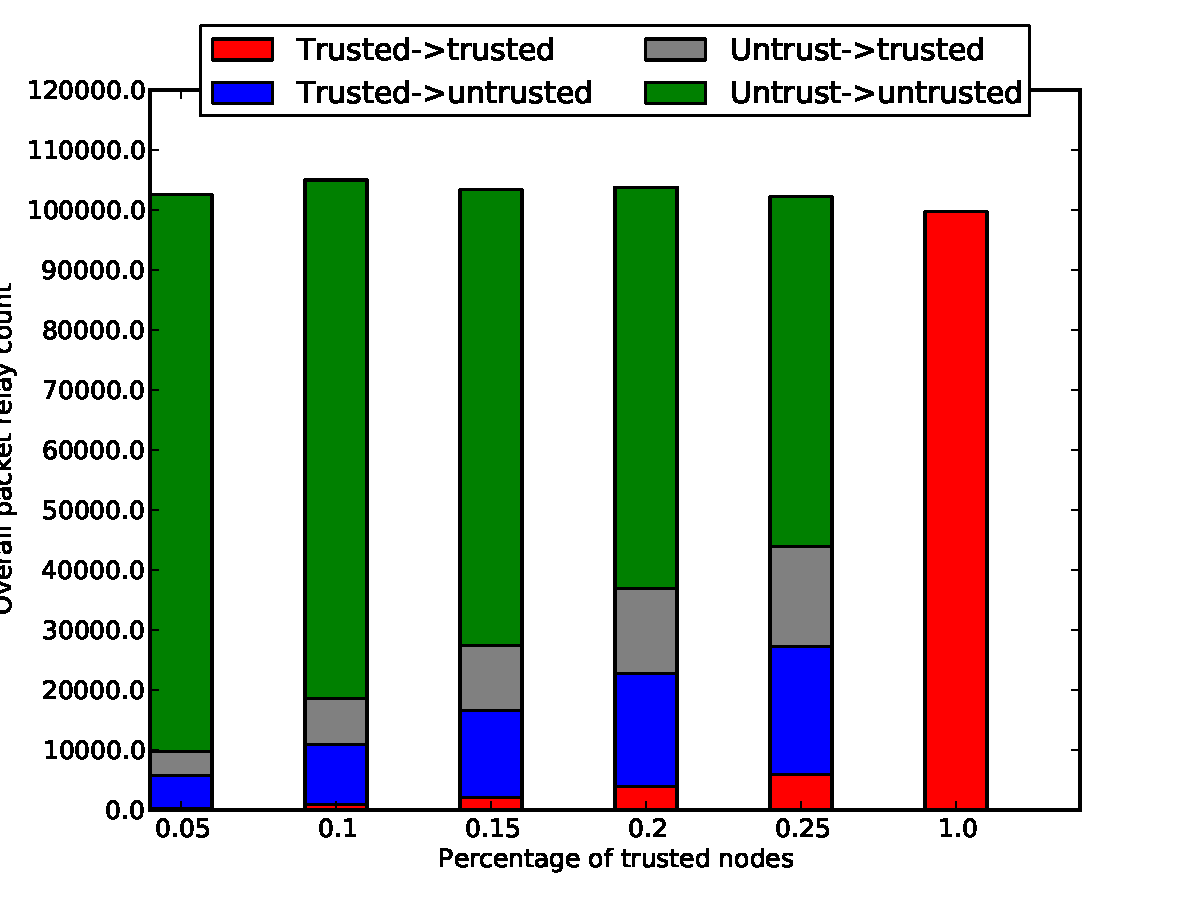
\includegraphics[width=0.33\columnwidth]{figures/epoch_6_maxbuffer/relay_classification_over_percentage.pdf}
\label{fig:relay_classification_percentage_6_maxbuffer}
}
\hfill
\subfloat[Delivered packets. Ephemeral ID valid for 3 epochs.]{%
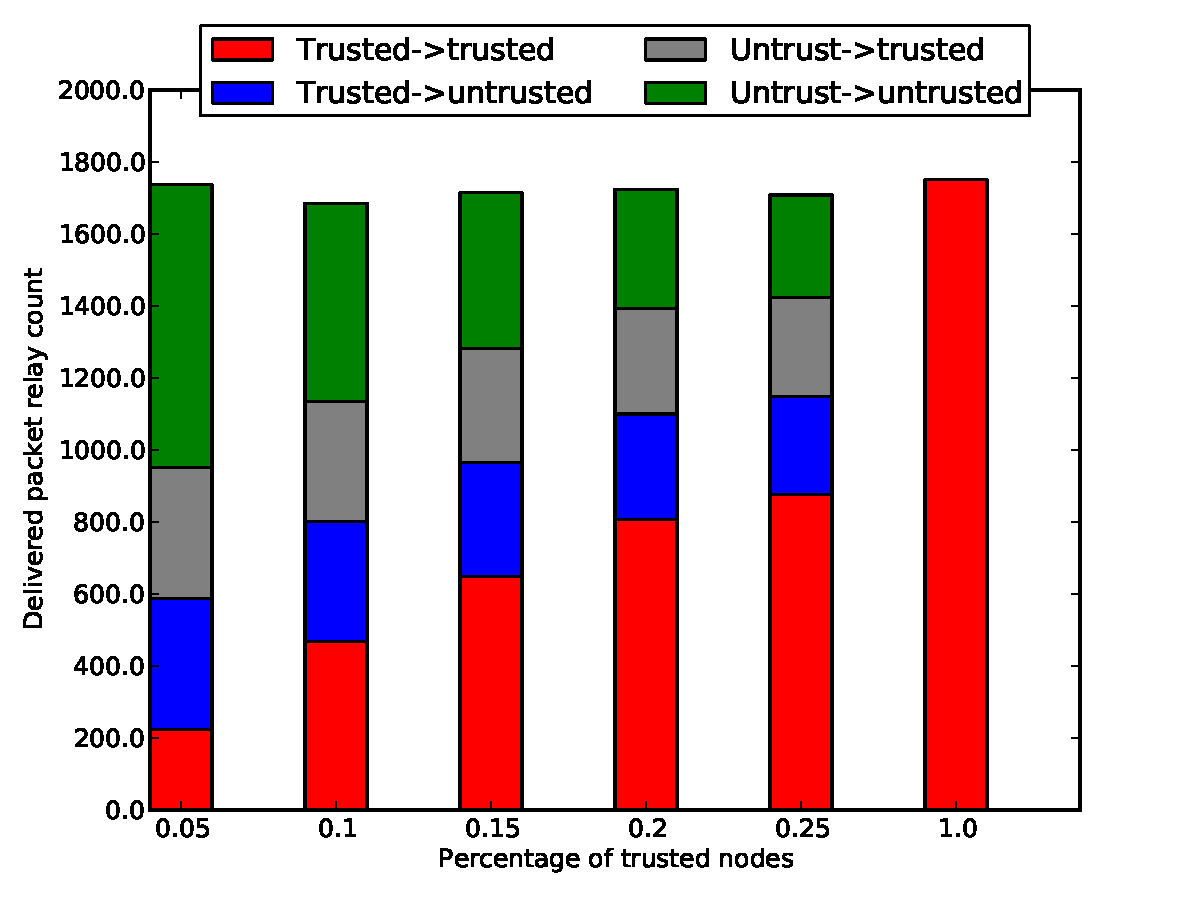
\includegraphics[width=0.33\columnwidth]{figures/epoch_3/relay_delivery_classification_over_percentage.pdf}
\label{fig:delivered_relay_classification_percentage_3}
}
%\hfill
\subfloat[Delivered packets. Ephemeral ID valid for 6 epochs.]{%{%
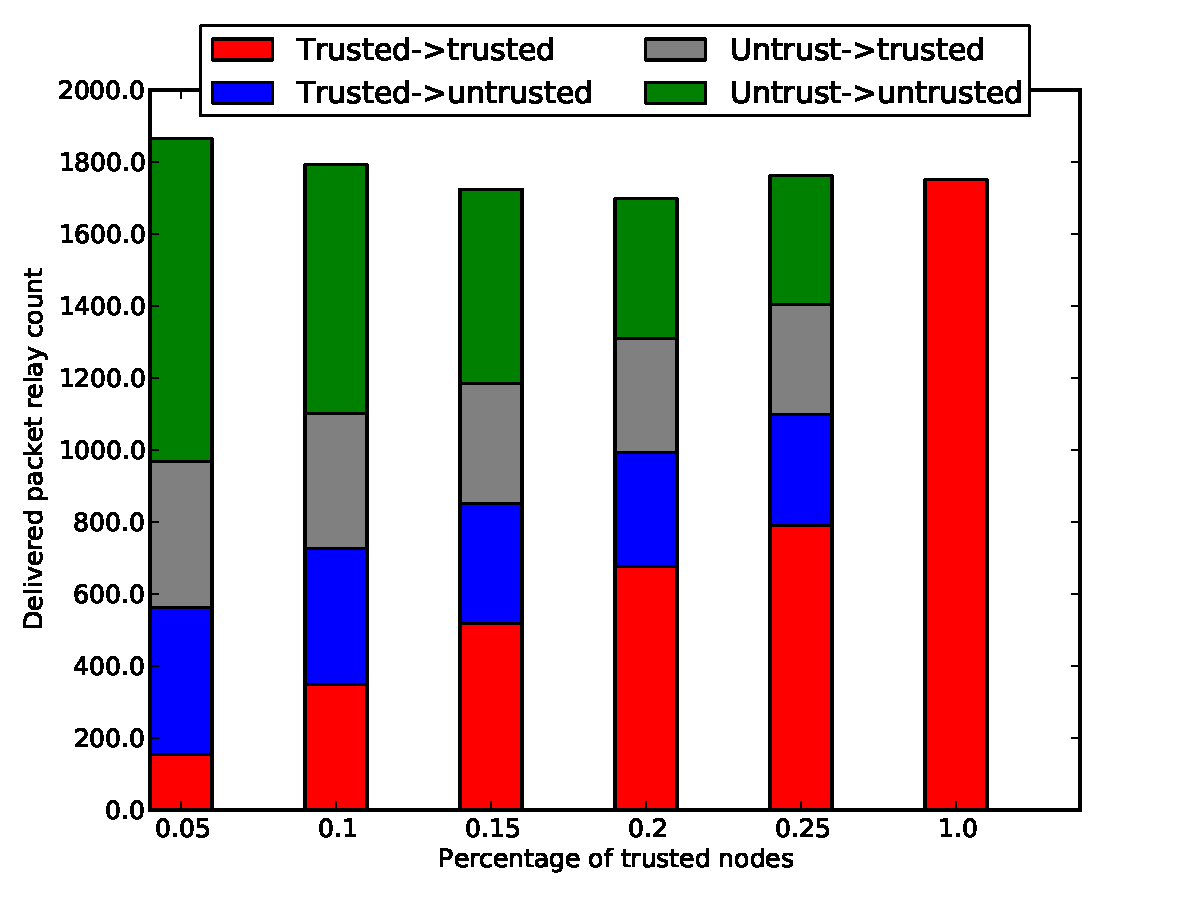
\includegraphics[width=0.33\columnwidth]{figures/epoch_6/relay_delivery_classification_over_percentage.pdf}
\label{fig:delivered_relay_classification_percentage_6}
}
%\hfill
\subfloat[Delivered packets. Ephemeral ID valid for 6 epochs. Infinite packet buffer]{%{%
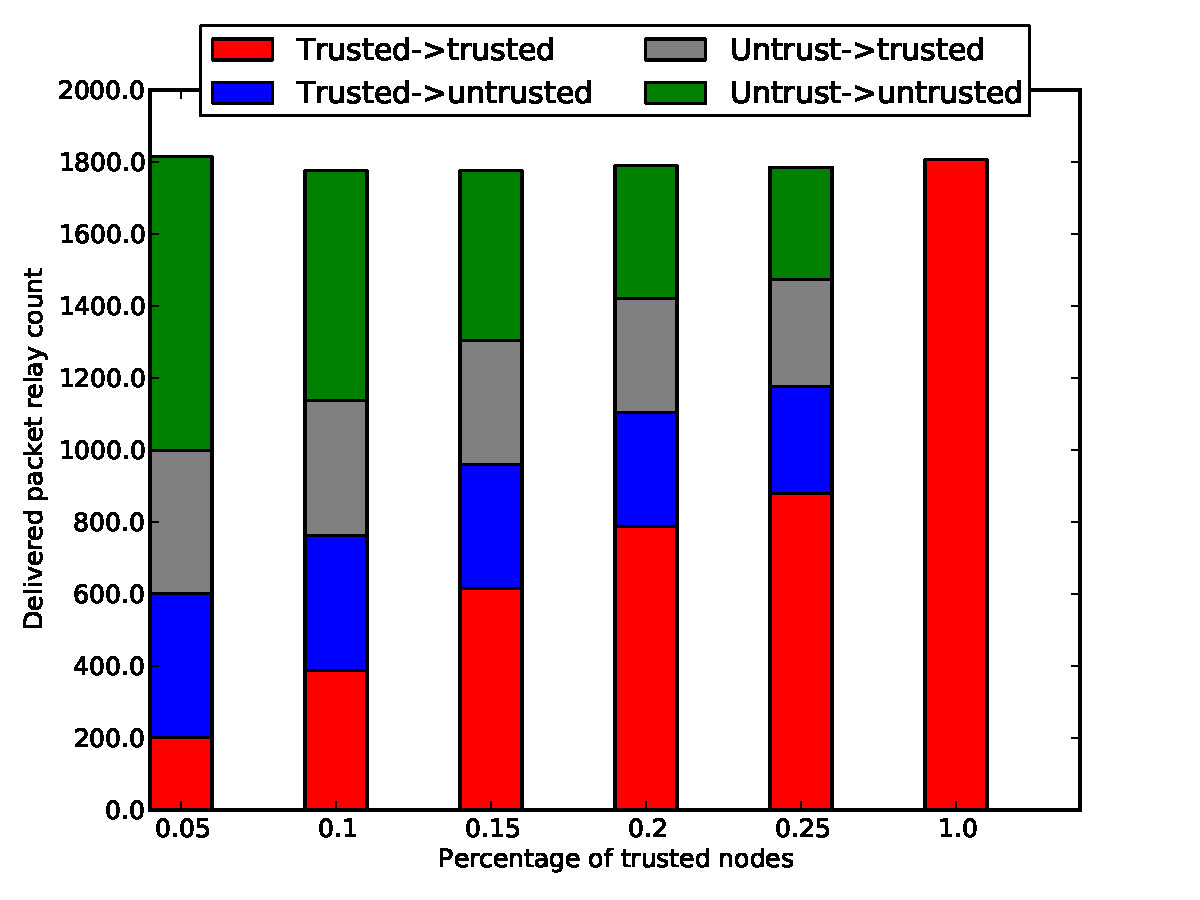
\includegraphics[width=0.33\columnwidth]{figures/epoch_6_maxbuffer/relay_delivery_classification_over_percentage.pdf}
\label{fig:delivered_relay_classification_percentage_6_maxbuffer}
}

\caption{{\bf Packet relay classification over varying percentage of trusted nodes. Epoch is $30$ mins.}
As in Figure~\ref{fig:relay_classification_epoch}, ephemeral ID duration does not affect overall packet relay classification but affects delivered packet relay classification. 
}
\label{fig:relay_classification_percentage}
\end{figure}






% packet drop classification
\begin{figure}[h!]
\center
\subfloat[Varying epochs. Percentage of trusted nodes = 15\%. Ephemeral ID valid for 3 epochs.]{%
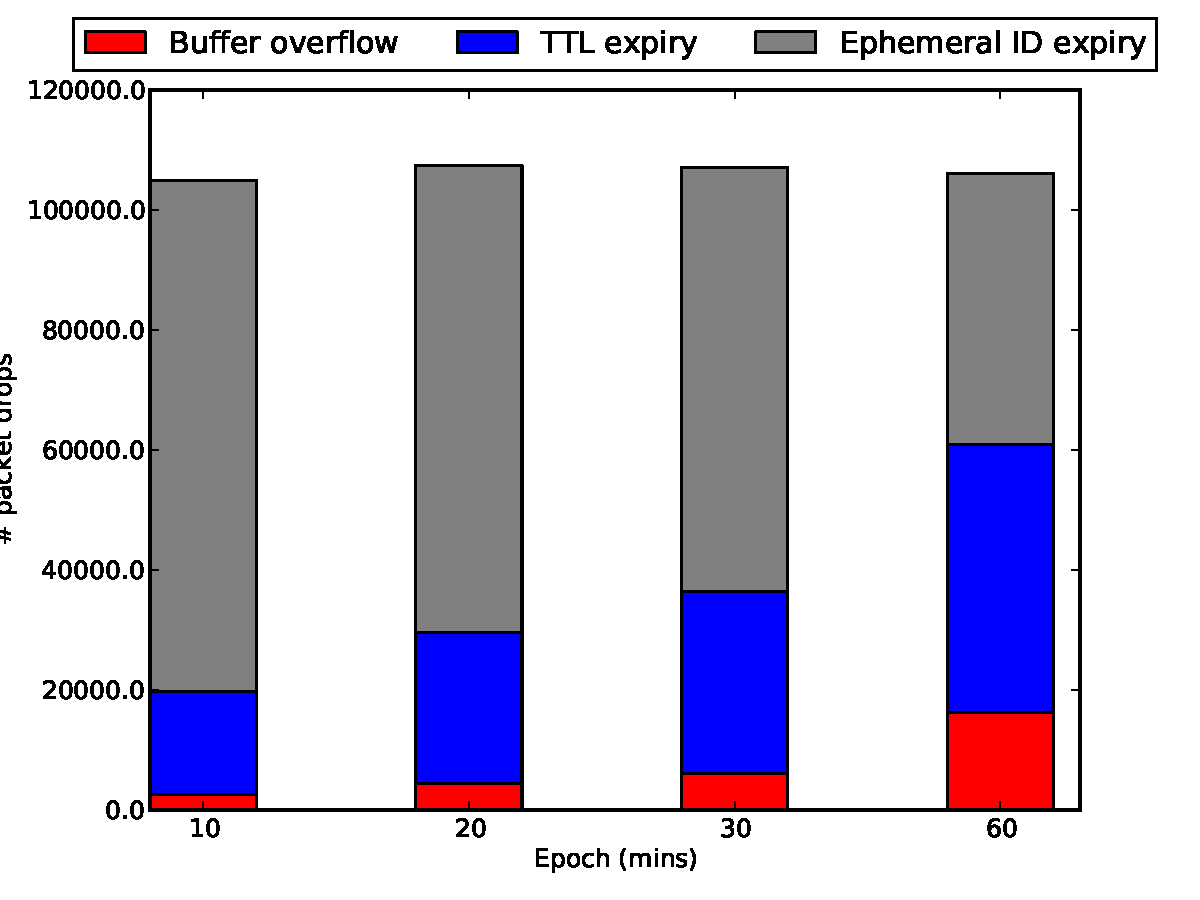
\includegraphics[width=0.33\columnwidth]{figures/epoch_3/drop_classification_over_epoch.pdf}
\label{fig:drop_classification_epoch_3}
}
%\hfill
\subfloat[Varying epochs. Percentage of trusted nodes = 15\%. Ephemeral ID valid for 6 epochs.]{%
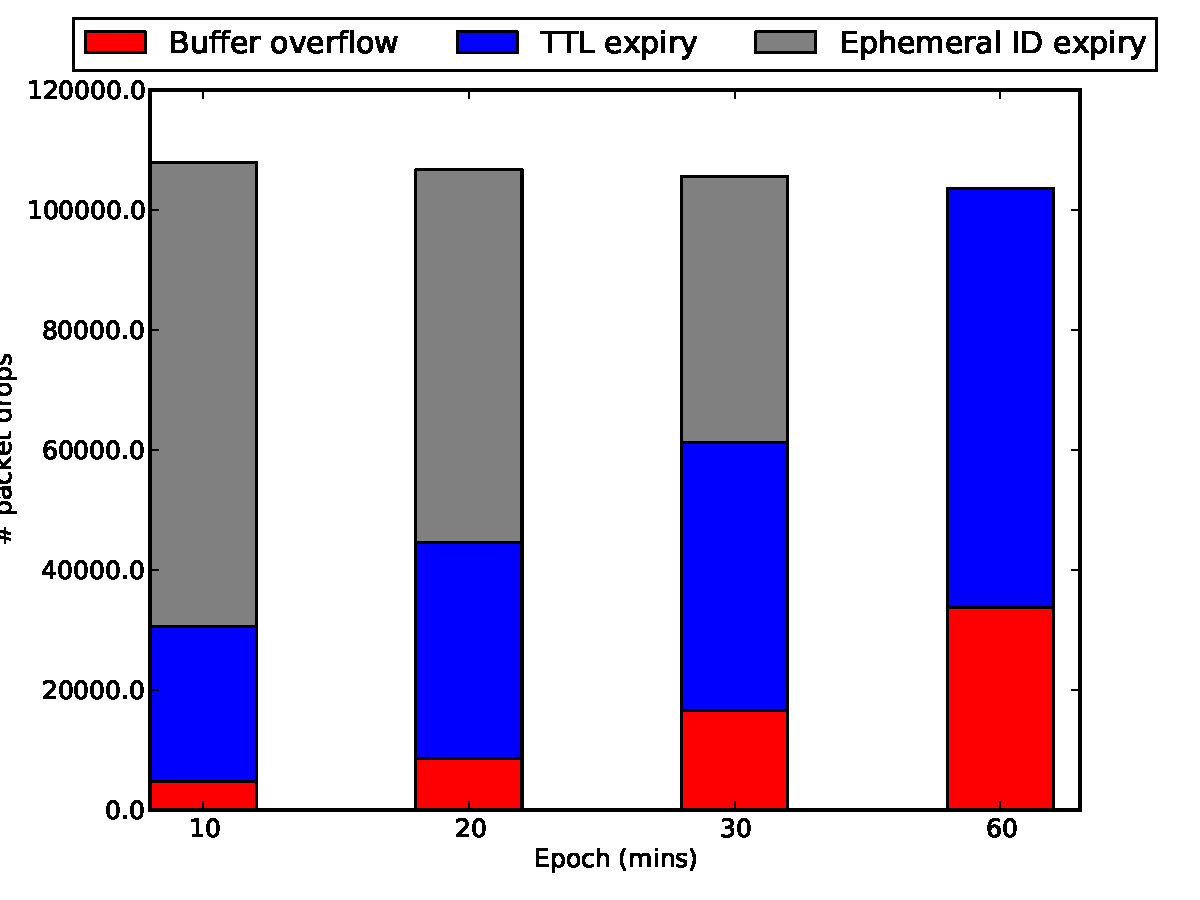
\includegraphics[width=0.33\columnwidth]{figures/epoch_6/drop_classification_over_epoch.pdf}
\label{fig:drop_classification_epoch_6}
}
\subfloat[Varying epochs. Percentage of trusted nodes = 15\%. Ephemeral ID valid for 6 epochs. Infinite packet buffer]{%
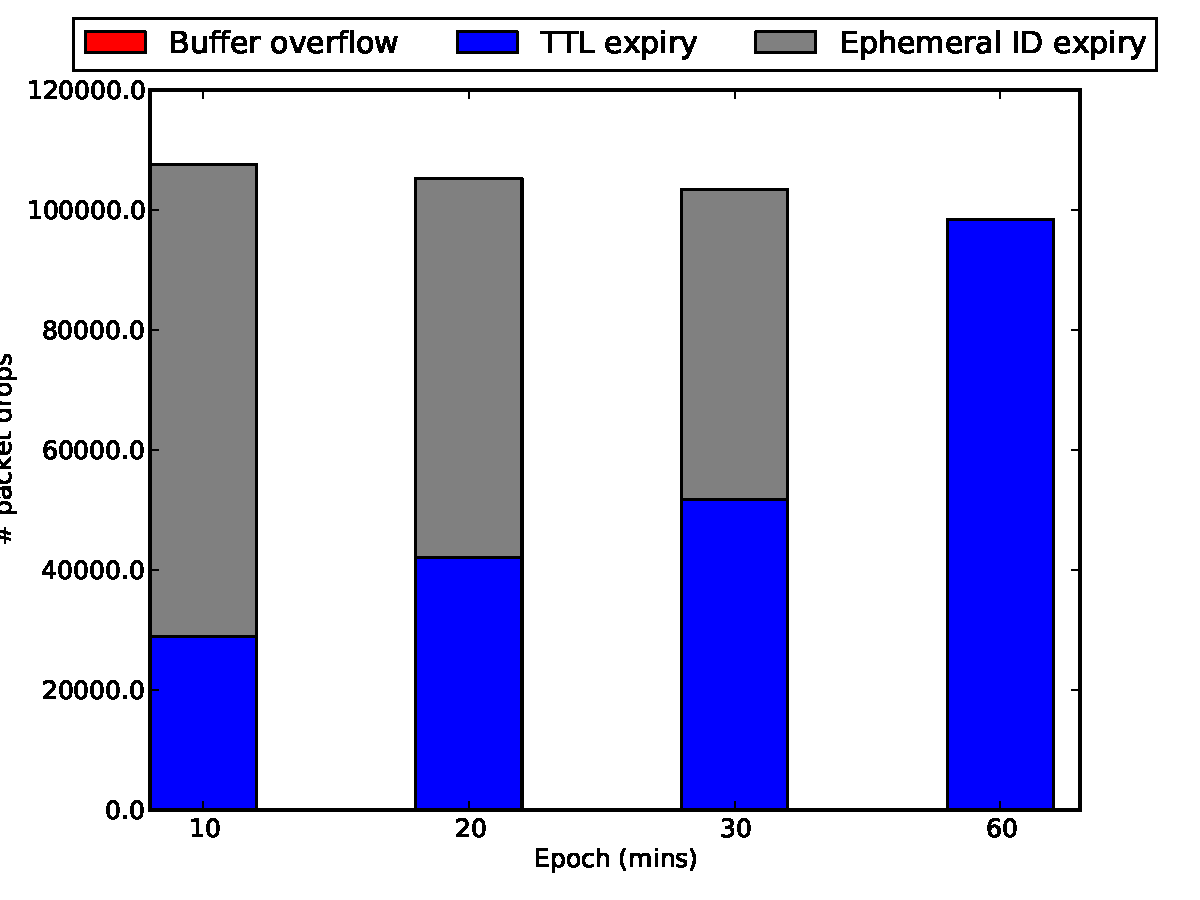
\includegraphics[width=0.33\columnwidth]{figures/epoch_6_maxbuffer/drop_classification_over_epoch.pdf}
\label{fig:drop_classification_epoch_6_maxbuffer}
}

\hfill
\subfloat[Varying percentage of trusted nodes. Epoch = 30 mins. Ephemeral ID valid for 3 epochs.]{%
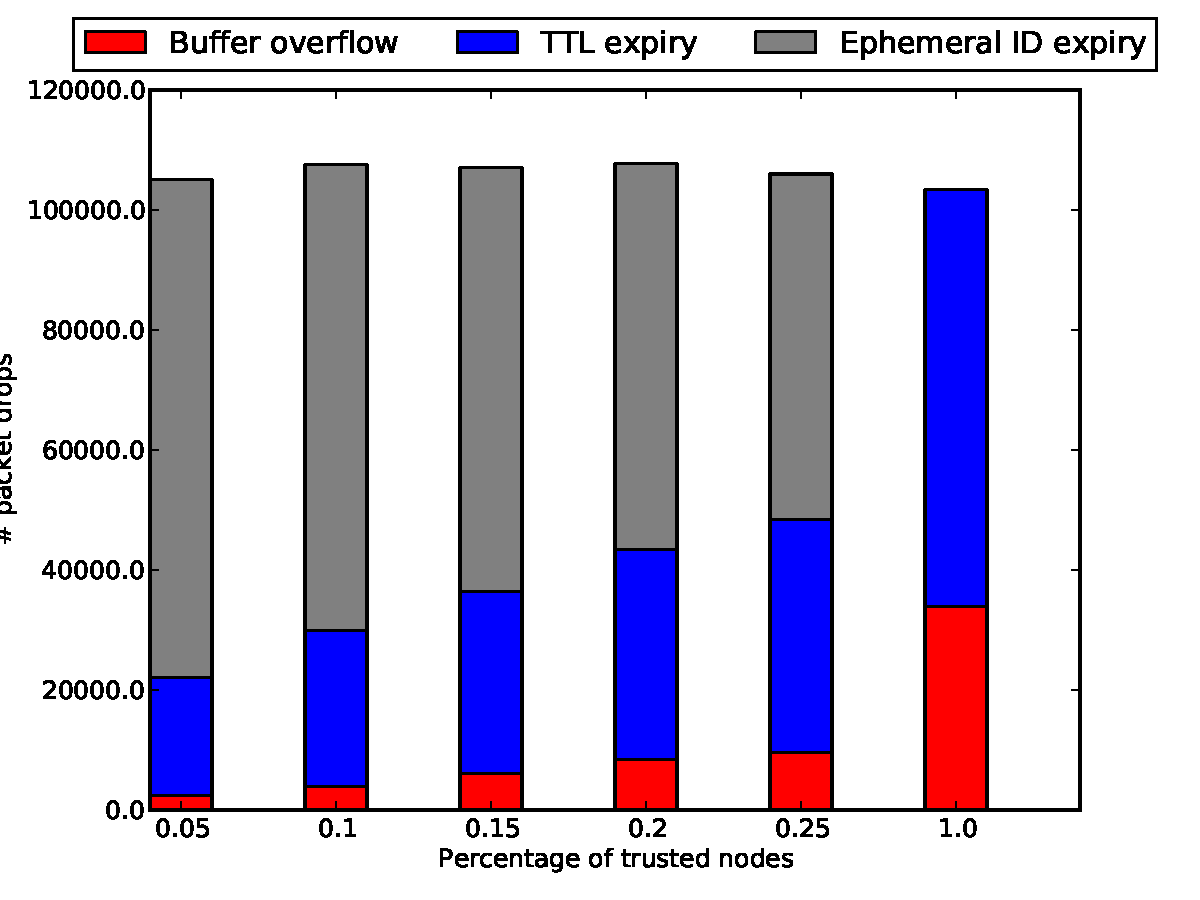
\includegraphics[width=0.33\columnwidth]{figures/epoch_3/drop_classification_over_percentage.pdf}
\label{fig:drop_classification_percentage_3}
}
\subfloat[Varying percentage of trusted nodes. Epoch = 30 mins. Ephemeral ID valid for 6 epochs.]{%
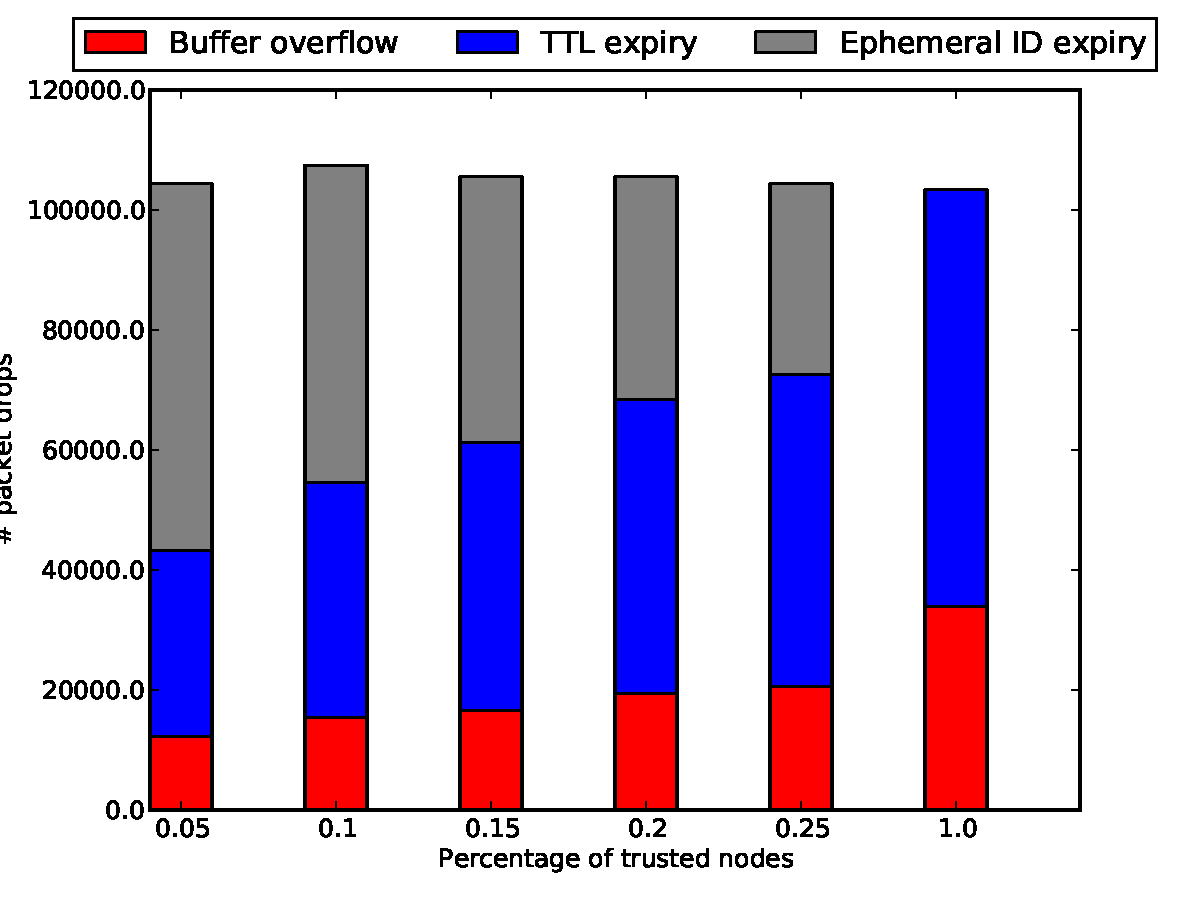
\includegraphics[width=0.33\columnwidth]{figures/epoch_6/drop_classification_over_percentage.pdf}
\label{fig:drop_classification_percentage_6}
}
\subfloat[Varying percentage of trusted nodes. Epoch = 30 mins. Ephemeral ID valid for 6 epochs. Infinite packet buffer.]{%
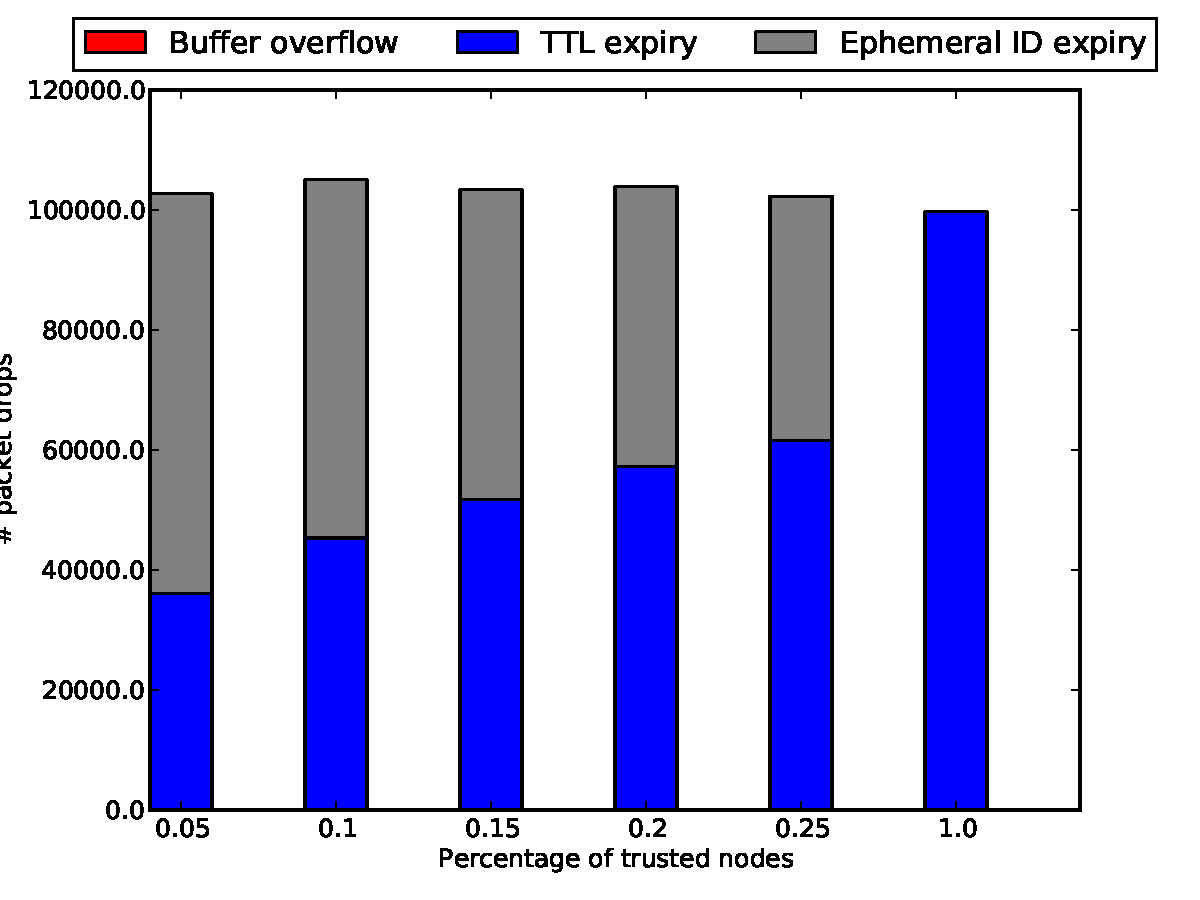
\includegraphics[width=0.33\columnwidth]{figures/epoch_6_maxbuffer/drop_classification_over_percentage.pdf}
\label{fig:drop_classification_percentage_6_maxbuffer}
}

\caption{{\bf Packet drop classification.}
With ephemeral ID valid for 6 epochs (Figures~\ref{fig:drop_classification_epoch_6} and \ref{fig:drop_classification_percentage_6}),  
packet drops due to ephemeral ID expiry are decreased significantly.
Note that packet drop due to ephemeral ID expiry does not occur when epoch is 60 mins and ephemeral ID duration is 6 epochs.  
[TTL (5 hours) $<$ Epoch (1 hour) * Ephemeral ID duration (6 epochs)]
}
\label{fig:drop_classification}
\end{figure}






% packet delivery count with untrusted nodes
\begin{figure}[t!]
\center
\subfloat[Ephemeral ID valid for 3 epochs.]{%
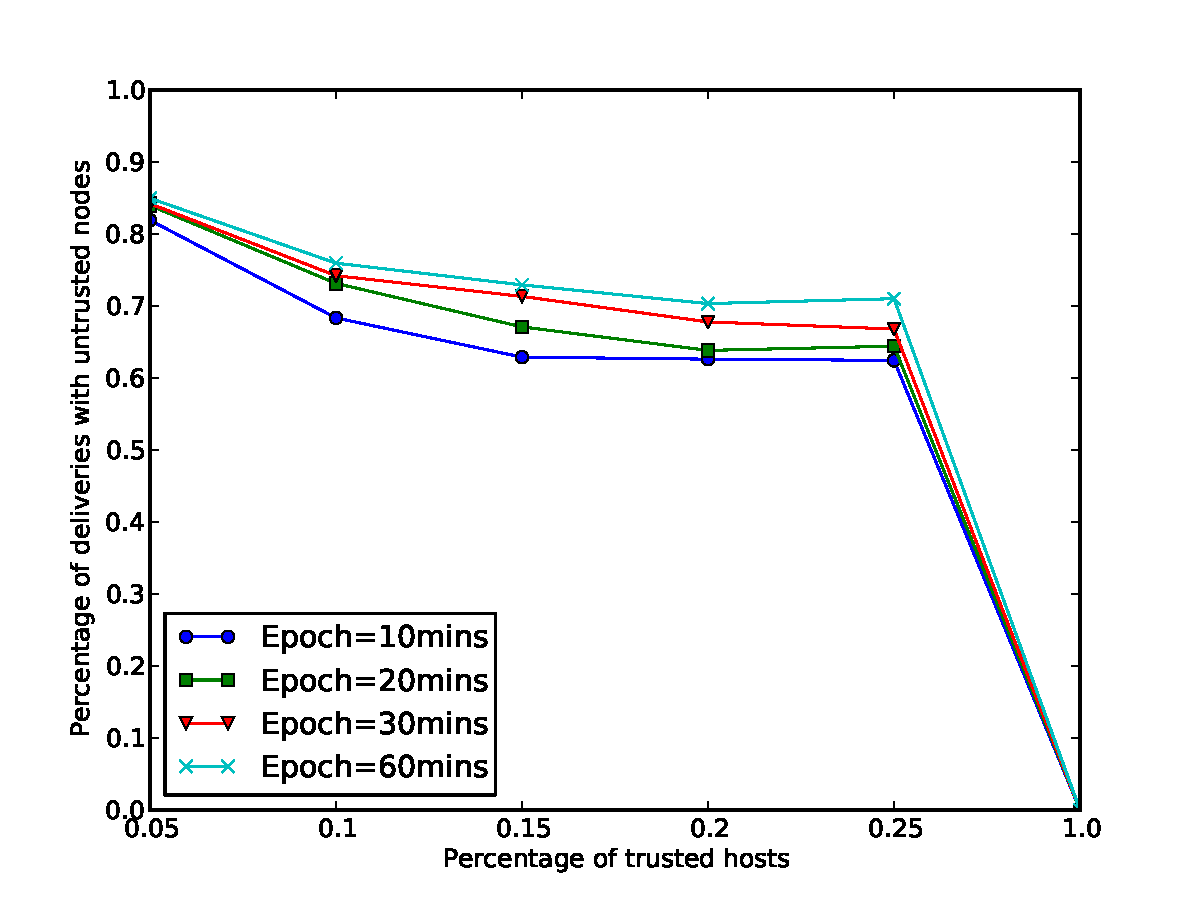
\includegraphics[width=0.33\columnwidth]{figures/epoch_3/delivery_with_ut.pdf}
\label{fig:delivery_ut_3}
}
%\hfill
\subfloat[Ephemeral ID valid for 6 epochs.]{%
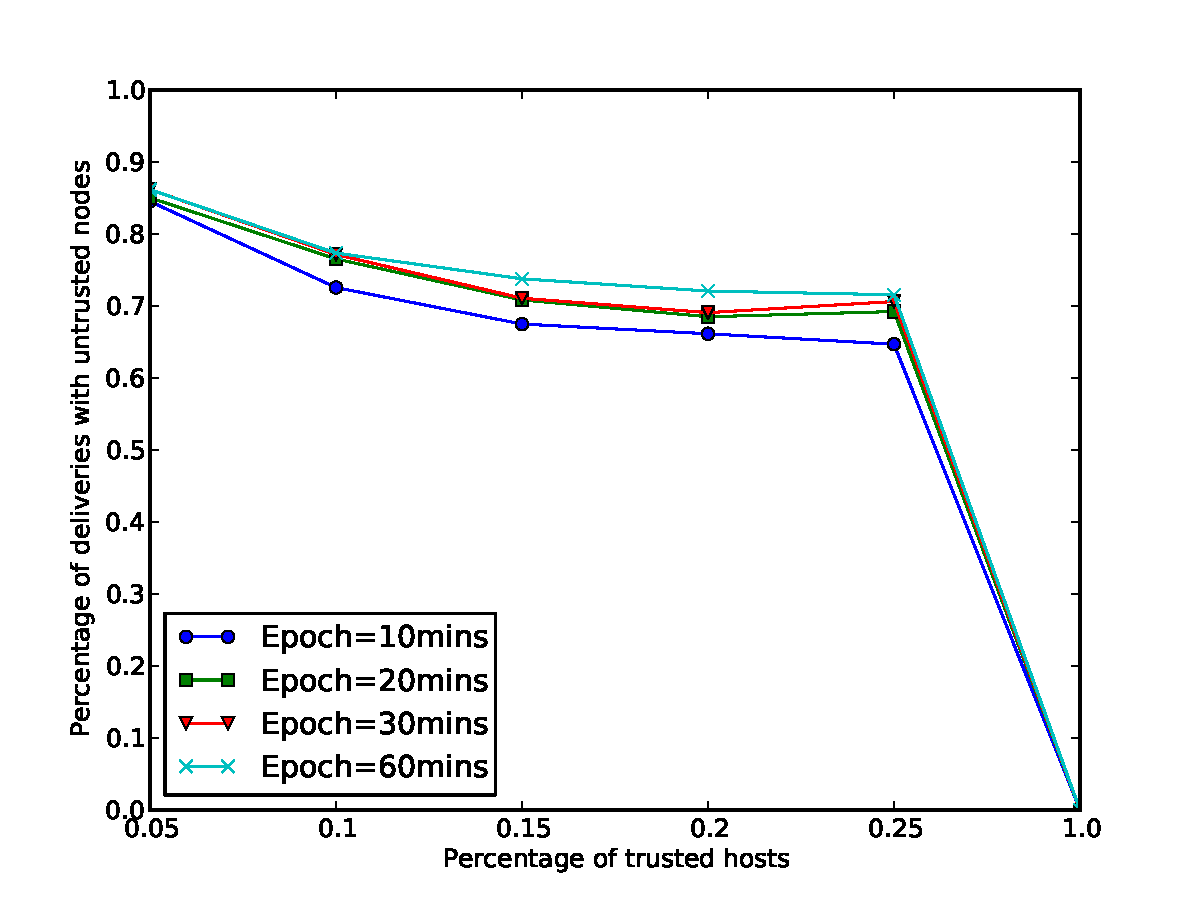
\includegraphics[width=0.33\columnwidth]{figures/epoch_6/delivery_with_ut.pdf}
\label{fig:delivery_ut_6}
}
\subfloat[Ephemeral ID valid for 6 epochs. Infinite packet buffer.]{%
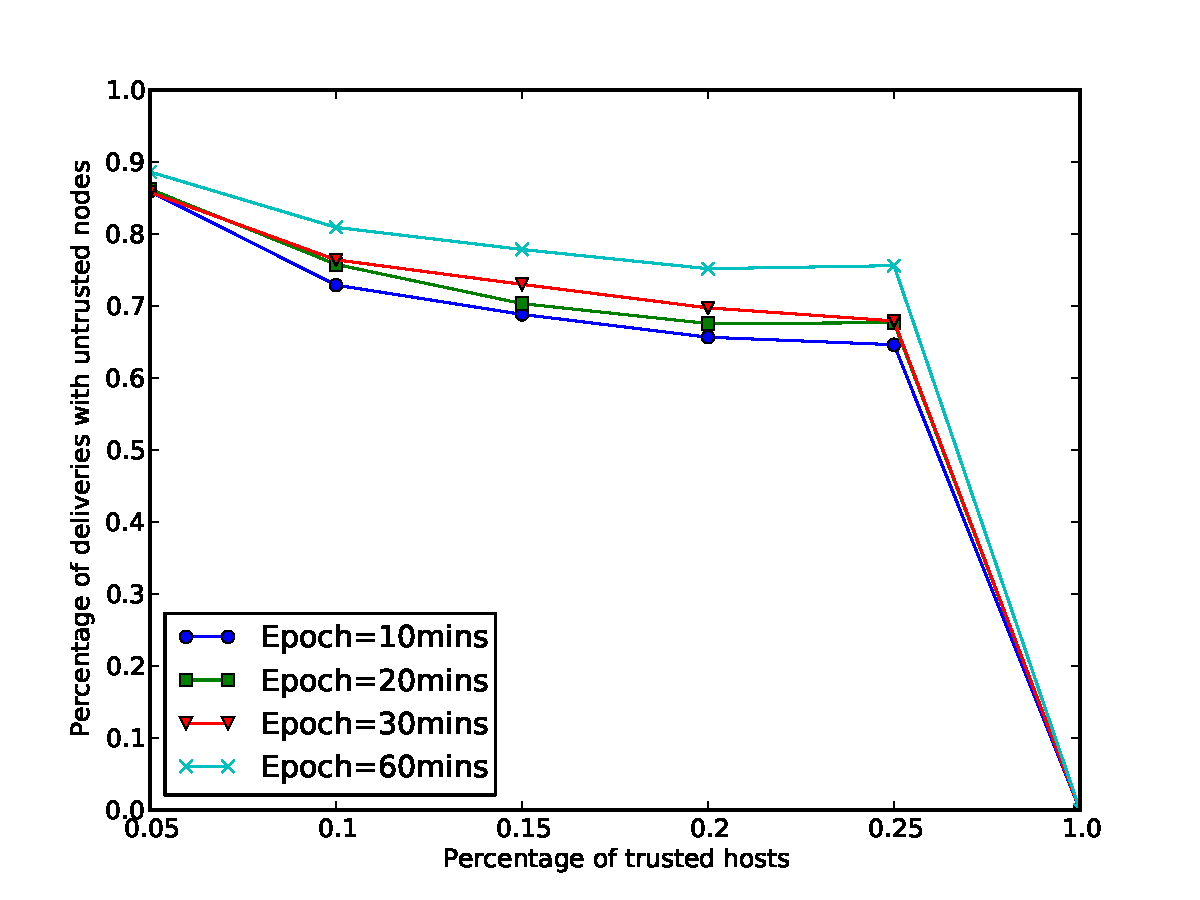
\includegraphics[width=0.33\columnwidth]{figures/epoch_6_maxbuffer/delivery_with_ut.pdf}
\label{fig:delivery_ut_6_maxbuffer}
}
\caption{{\bf Packet deliveries with untrusted nodes.} Percentage of packet delivery routes containing at least one untrusted node.}
\label{fig:delivery_count}
\end{figure}






\begin{comment}
% average relay count per message
\begin{figure}[h!]
\center
\subfloat[Average relay count per message. Ephemeral ID valid for 1 epoch]{%
\includegraphics[width=0.49\columnwidth]{figures/epoch_3/relay_per_message.pdf}
\label{fig:relay_per_message_3}
}
\hfill
\subfloat[Average relay count per message. Ephemeral ID valid for 3 epochs]{%
\includegraphics[width=0.49\columnwidth]{figures/epoch_6/relay_per_message.pdf}
\label{fig:relay_per_message_6}
}
\caption{{\bf Average relay counts per message.}
With ephemeral ID valid for 1 epoch, packets are not relayed enough times since the packets are dropped mainly due to ephemeral ID expiry, especially when the percentage of trusted node is low (Figure~\ref{fig:relay_per_message_3}). 
By using ephemeral ID valid for 3 epochs, the average relay count per message stays almost same regardless of the percentage of trusted nodes.
}
\label{fig:relay_per_message}
\end{figure}
\end{comment}

























\clearpage
\subsubsection{Communication among all nodes}
In this test scenario, every node can send packets to any other nodes.
Packet generation follows rules below:
\begin{itemize}
\item Nodes belong to the group generate and receive about 20\% of overall packets generated during the simulation. 
\item For the rest 80\% of packet generation, sender and receiver are randomly selected from all node. 
\end{itemize}



\begin{table}[!h]
\center
\begin{tabular}[!h]{|c|c|c|}
\hline
Ephemeral ID duration	& Trusted nodes \%	& Epoch	\\	
\hline
\hline
\multirow{2}{*}{3 epochs}	& 5\%				& 60 mins	\\
							& 10\%				& 30 mins	\\
\hline
\multirow{2}{*}{6 epochs}	& 5\%			& 30 mins \\
							& 10\%			& 20 mins \\
\hline
\end{tabular}
\vspace{10pt}
\caption{{ \bf Example settings with overall delivery rate of about 90\% (Flooding: 92.91\%).}}
\label{tab:dataset_summary}
\end{table}




% delivery rate
\begin{figure}[h!]
\center
\subfloat[Ephemeral ID valid for 3 epochs]{%
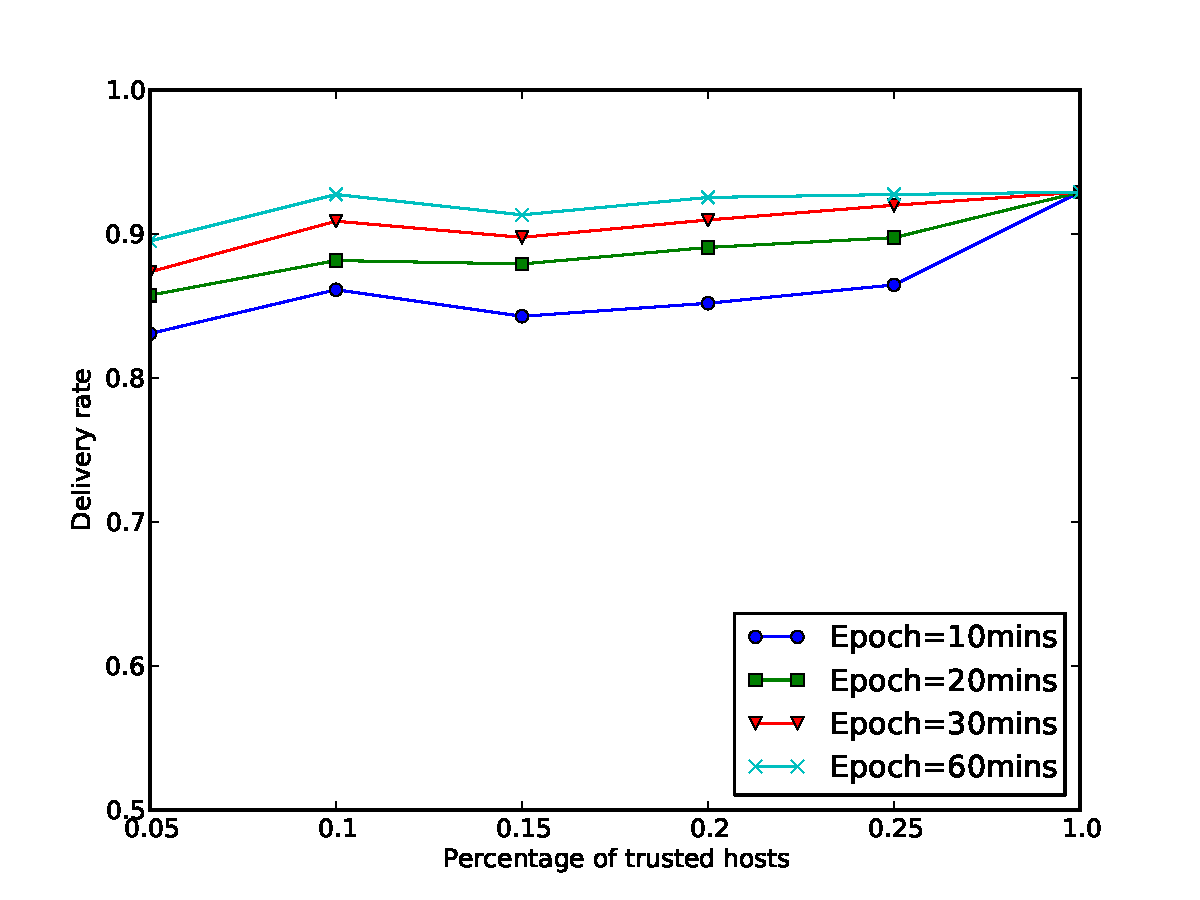
\includegraphics[width=0.49\columnwidth]{figures/epoch_3_overall/delivery_rate.pdf}
\label{fig:delivery_rate_3_overall}
}
\hfill
\subfloat[Ephemeral ID valid for 6 epochs]{%
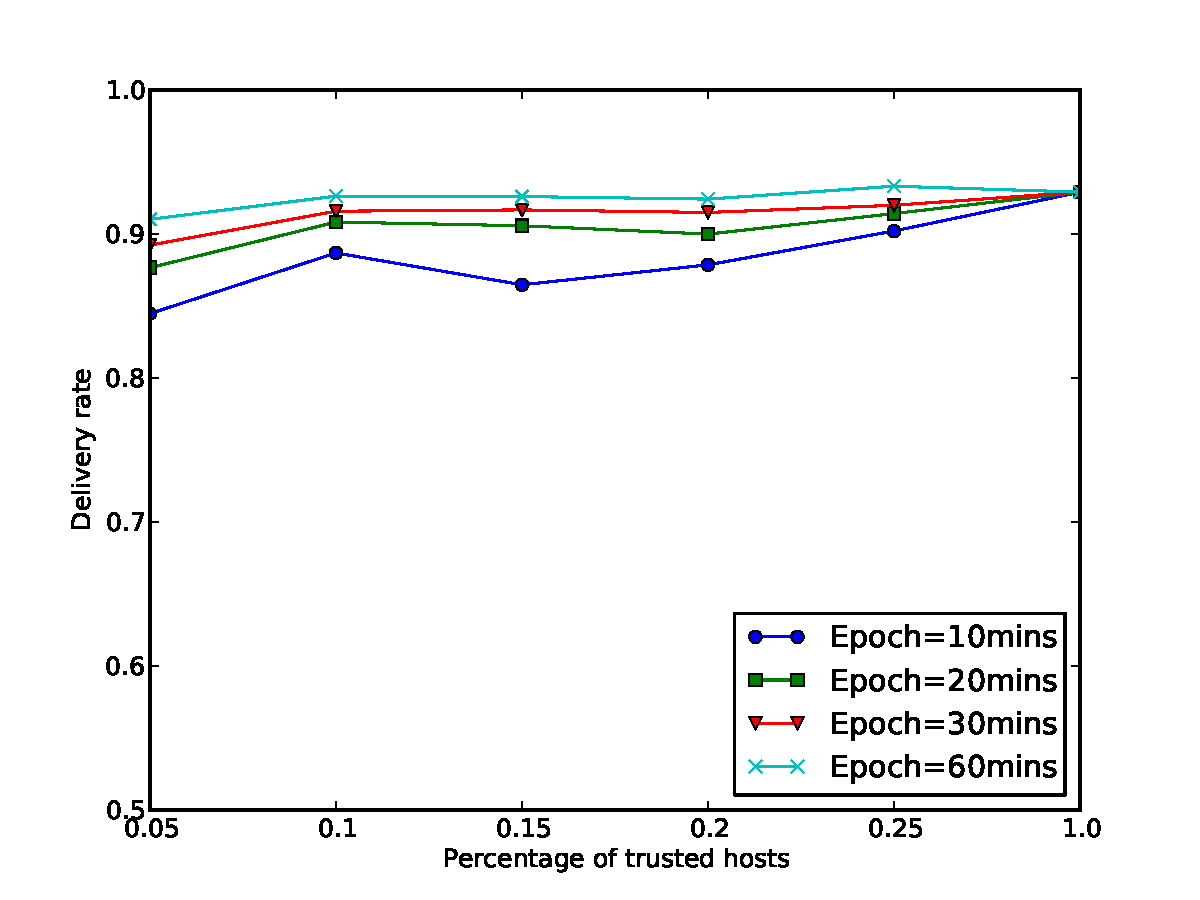
\includegraphics[width=0.49\columnwidth]{figures/epoch_6_overall/delivery_rate.pdf}
\label{fig:delivery_rate_6_overall}
}

\caption{{\bf Overall packet delivery rate.} 
Delivery rate of pure epidemic routing: 92.91\%.  
With epoch=60 mins, overall delivery rate is almost similar to that of epidemic routing regardless of the percentage of trusted nodes. 
In Figure~\ref{fig:delivery_rate_6_overall}, delivery rates with epoch $\ge$ 20 mins are about 90\%, especially when the percentage of trusted nodes $\ge 10\%$.
}
\label{fig:delivery_rate}
\end{figure}



% delivery rate retails
\begin{figure}[h!]
\center
\subfloat[In-group to In-group. Ephemeral ID valid for 3 epochs]{%
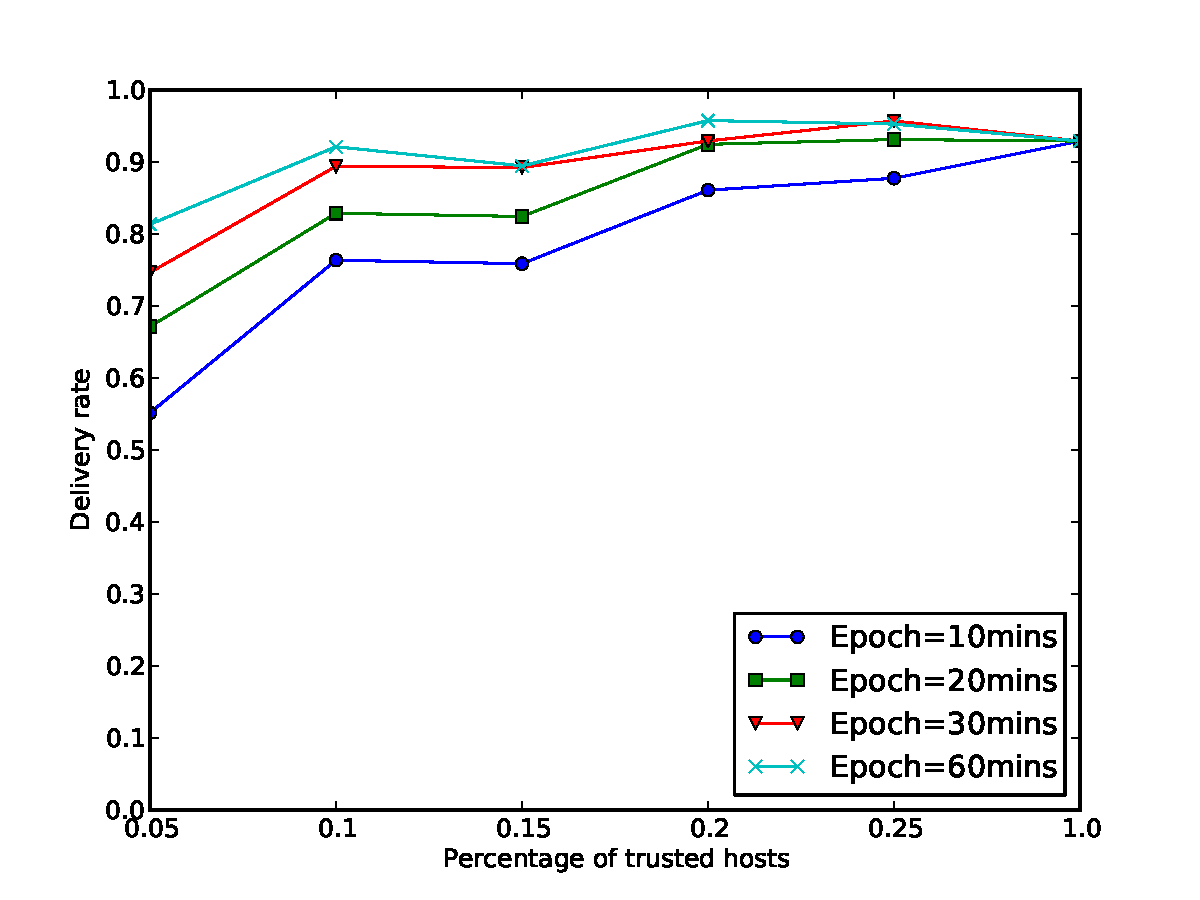
\includegraphics[width=0.33\columnwidth]{figures/epoch_3_overall/delivery_rate_t_to_t.pdf}
\label{fig:delivery_rate_3_t_to_t}
}
\subfloat[In-group to In-group. Ephemeral ID valid for 6 epochs]{%
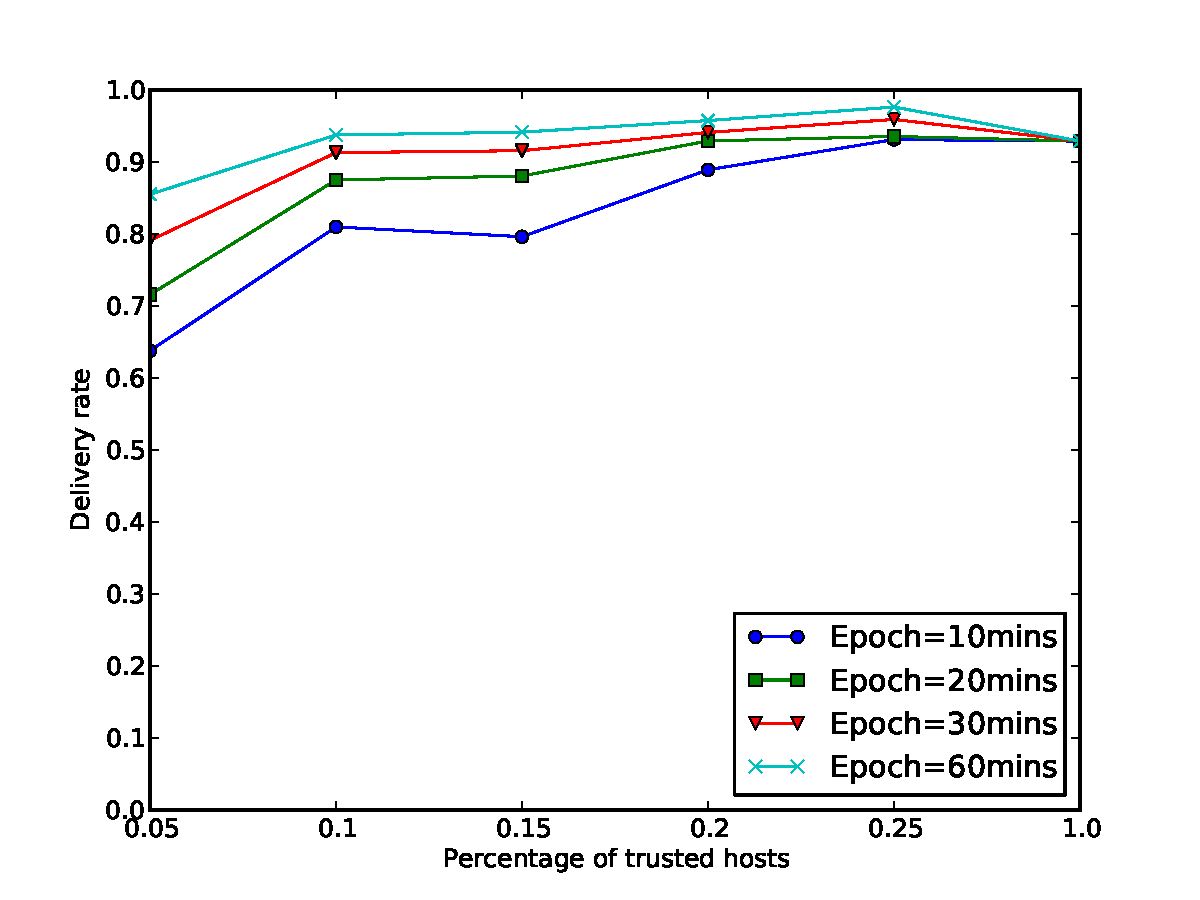
\includegraphics[width=0.33\columnwidth]{figures/epoch_6_overall/delivery_rate_t_to_t.pdf}
\label{fig:delivery_rate_6_t_to_t}
}
\hfill

\subfloat[In-group to Out-of-group. Ephemeral ID valid for 3 epochs]{%
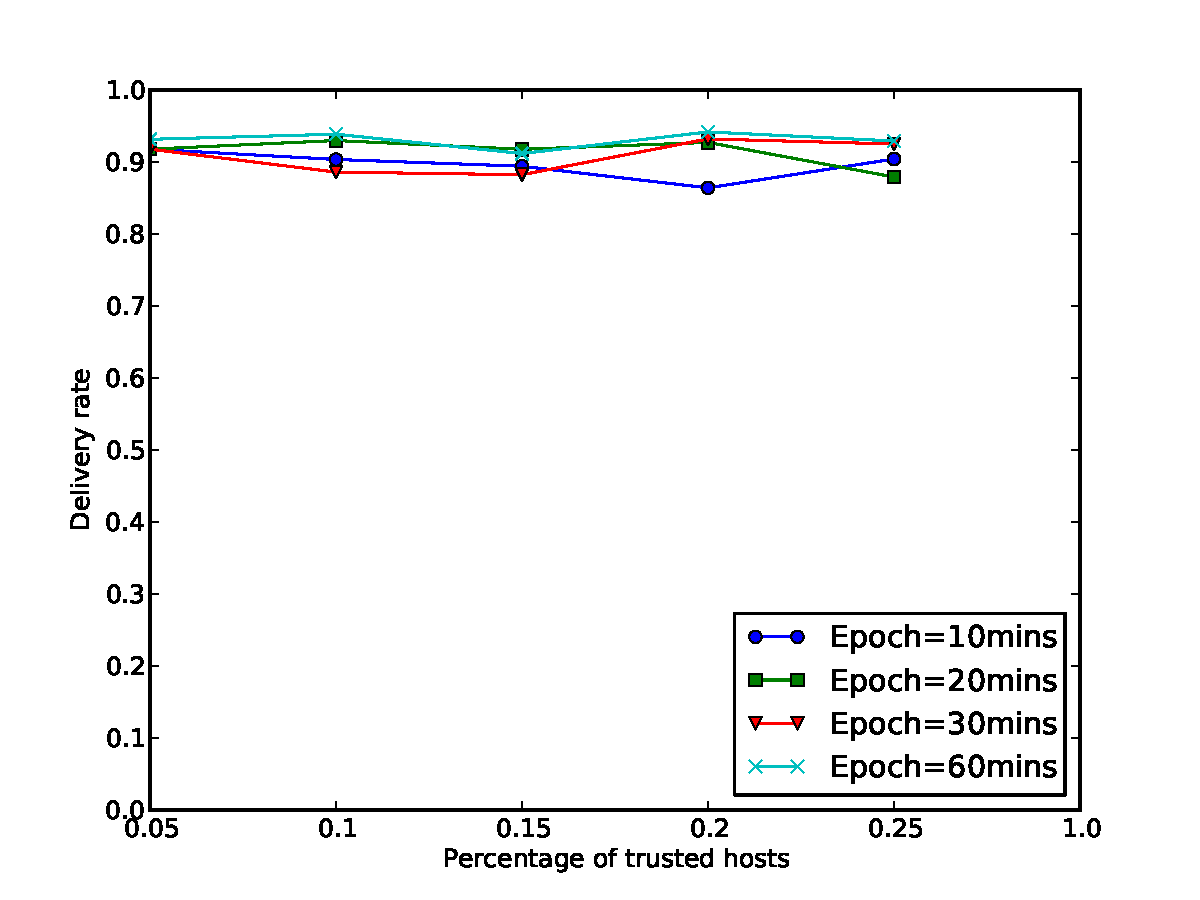
\includegraphics[width=0.33\columnwidth]{figures/epoch_3_overall/delivery_rate_t_to_ut.pdf}
\label{fig:delivery_rate_3_t_to_ut}
}
\subfloat[In-group to Out-of-group. Ephemeral ID valid for 6 epochs]{%
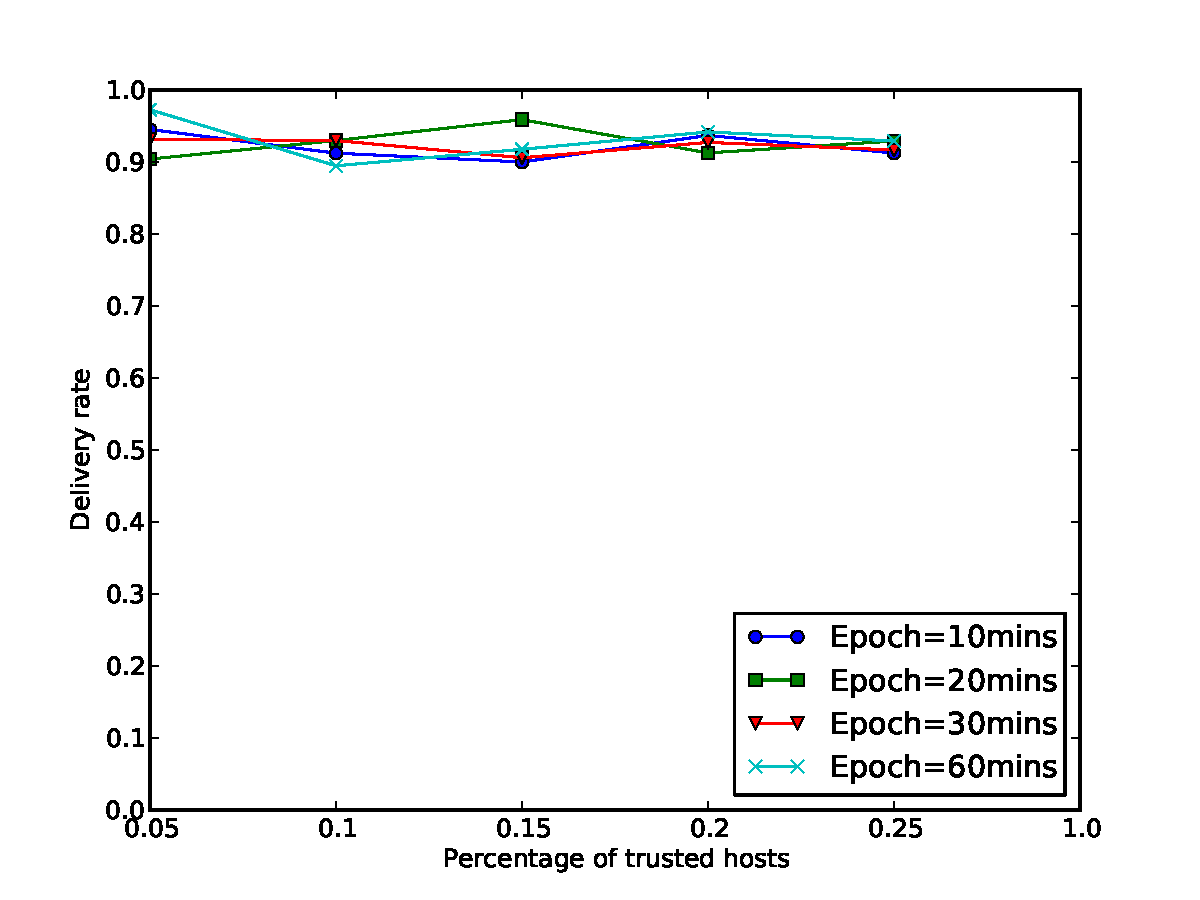
\includegraphics[width=0.33\columnwidth]{figures/epoch_6_overall/delivery_rate_t_to_ut.pdf}
\label{fig:delivery_rate_6_t_to_ut}
}
\hfill

\subfloat[Out-of-group to In-group. Ephemeral ID valid for 3 epochs]{%
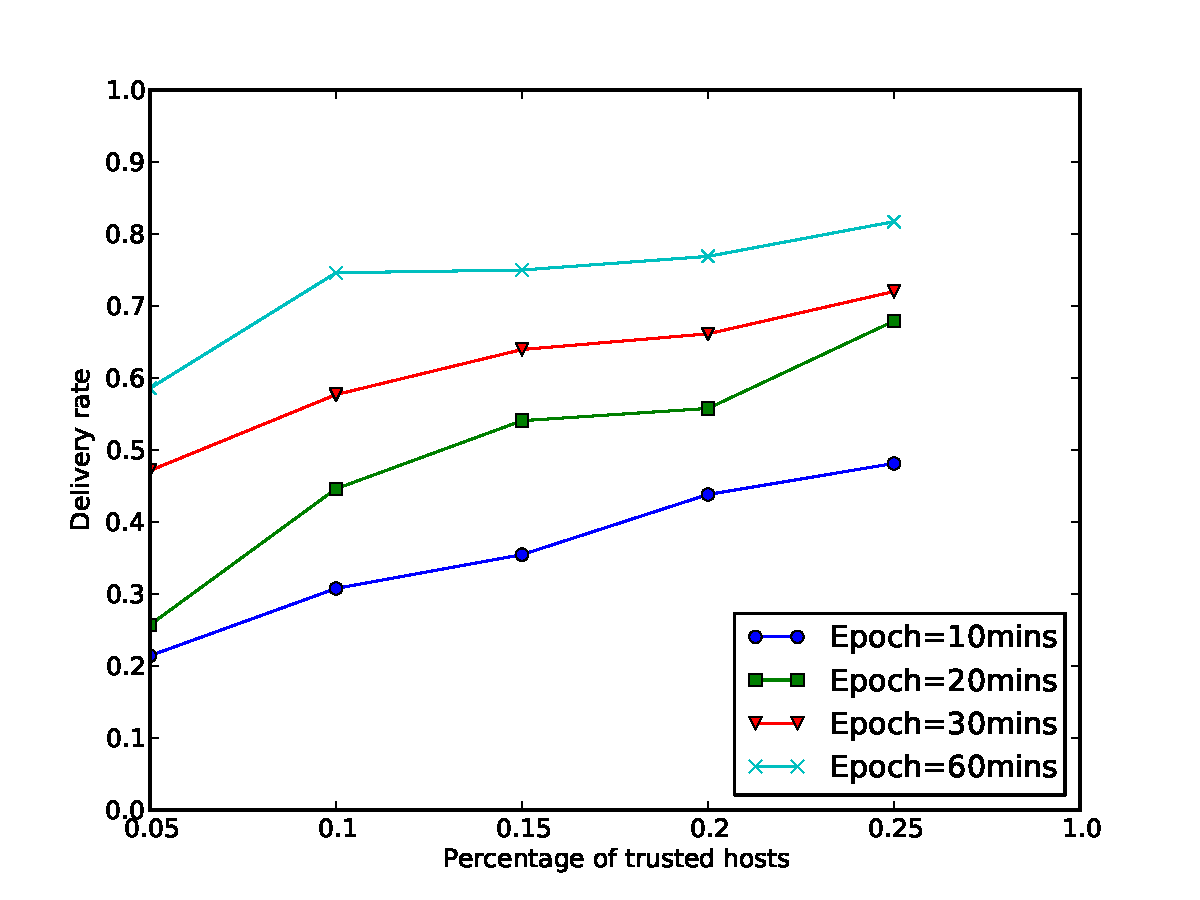
\includegraphics[width=0.33\columnwidth]{figures/epoch_3_overall/delivery_rate_ut_to_t.pdf}
\label{fig:delivery_rate_3_ut_to_t}
}
\subfloat[Out-of-group to In-group. Ephemeral ID valid for 6 epochs]{%
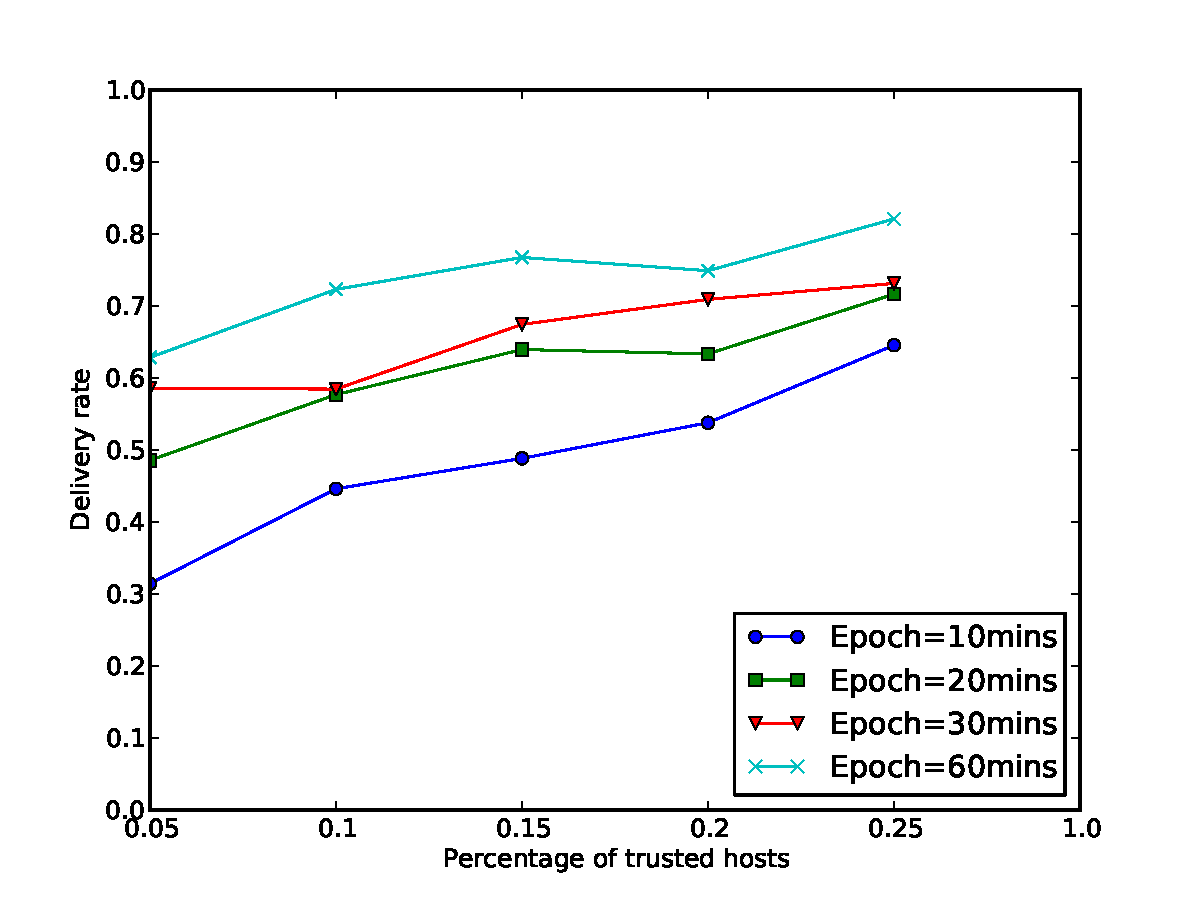
\includegraphics[width=0.33\columnwidth]{figures/epoch_6_overall/delivery_rate_ut_to_t.pdf}
\label{fig:delivery_rate_6_ut_to_t}
}
\hfill

\subfloat[Out-of-group to Out-of-group. Ephemeral ID valid for 3 epochs]{%
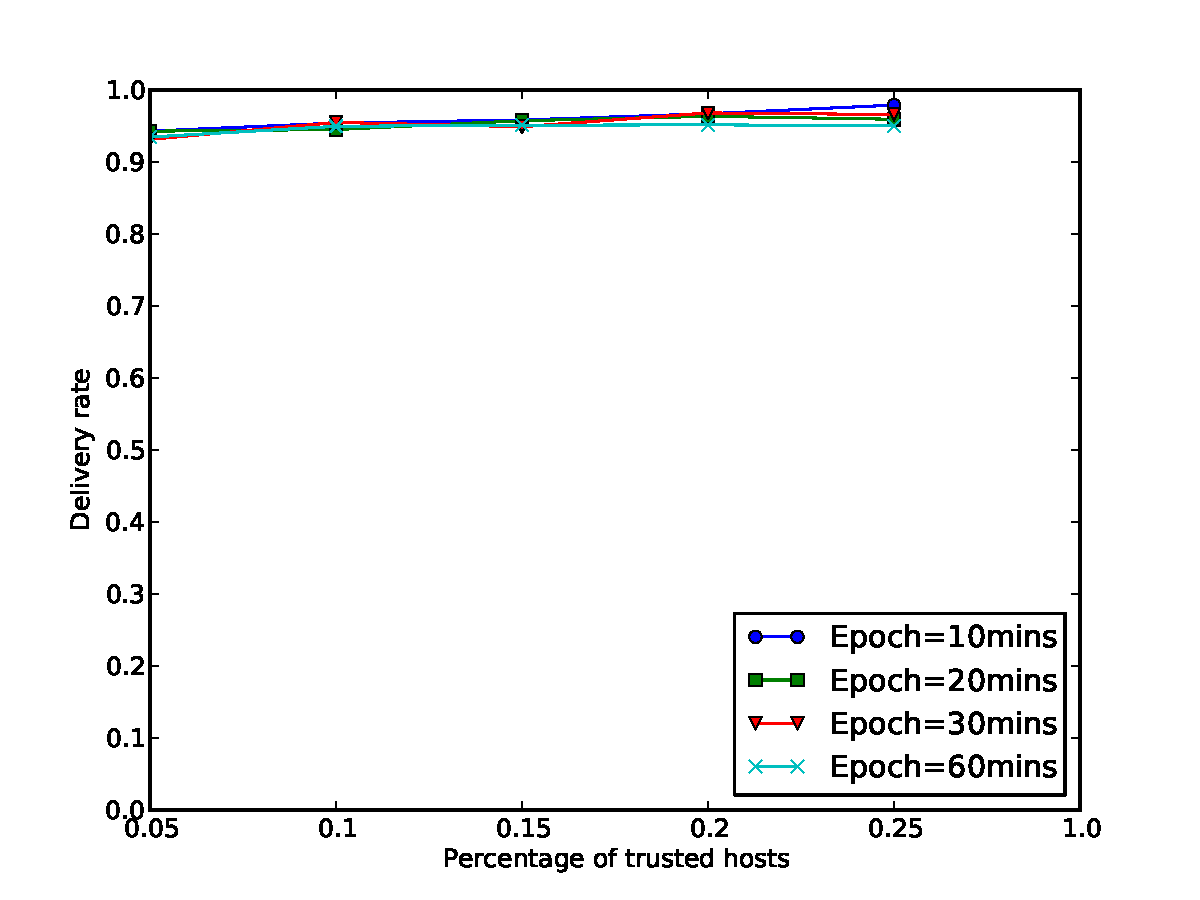
\includegraphics[width=0.33\columnwidth]{figures/epoch_3_overall/delivery_rate_ut_to_ut.pdf}
\label{fig:delivery_rate_3_ut_to_ut}
}
\subfloat[Out-group to Out-group. Ephemeral ID valid for 6 epochs]{%
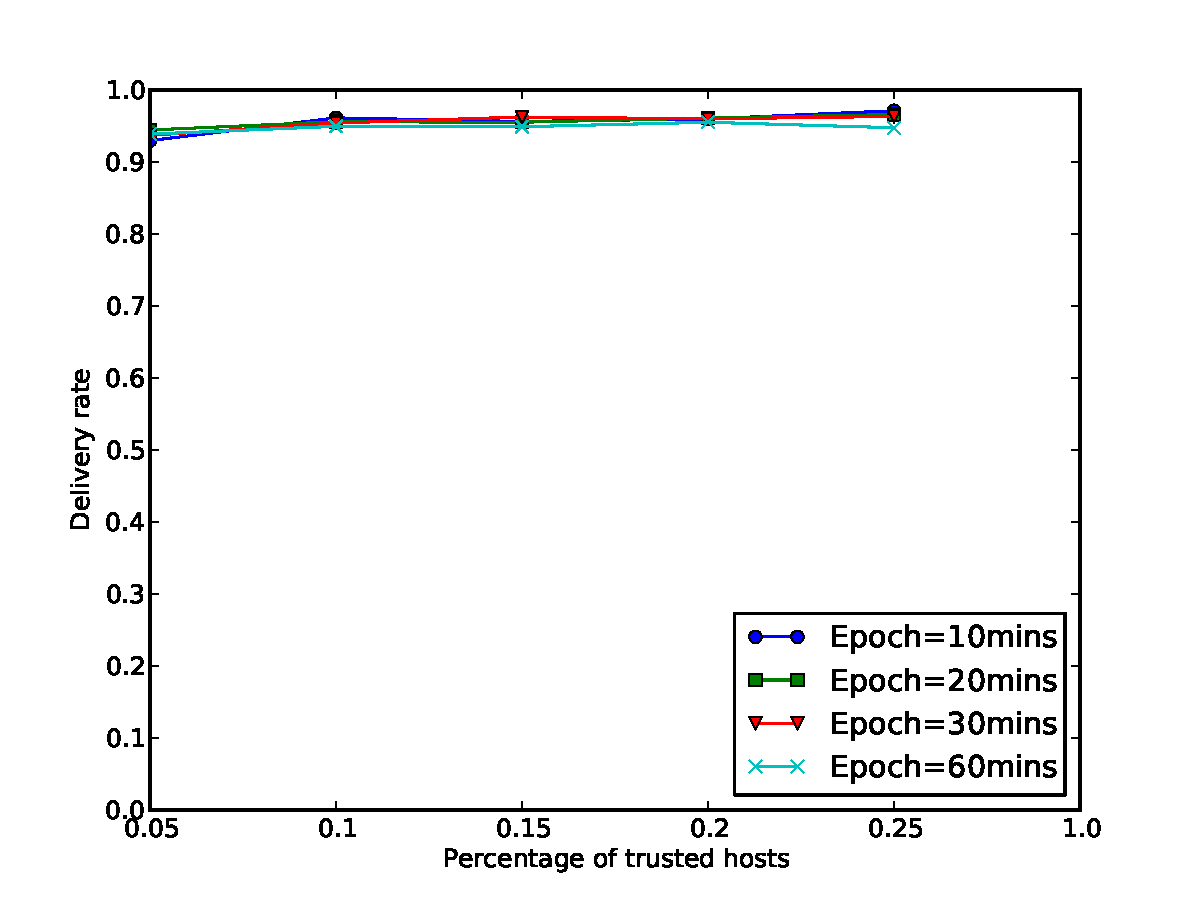
\includegraphics[width=0.33\columnwidth]{figures/epoch_6_overall/delivery_rate_ut_to_ut.pdf}
\label{fig:delivery_rate_6_ut_to_ut}
}

\caption{{\bf Detailed packet delivery rate.} 
Delivery rate of packets destined for `out-of-group' is almost same to that of epidemic routing, regardless of epoch and percentage of trusted nodes. 
Delivery rate of `Out-of-group' to `In-group' is relatively low, ranging from 20\% to 80\%. 
}
\label{fig:delivery_rate}
\end{figure}





% delivery latency
\begin{figure}[h!]
\center
\subfloat[Ephemeral ID valid for 3 epoch]{%
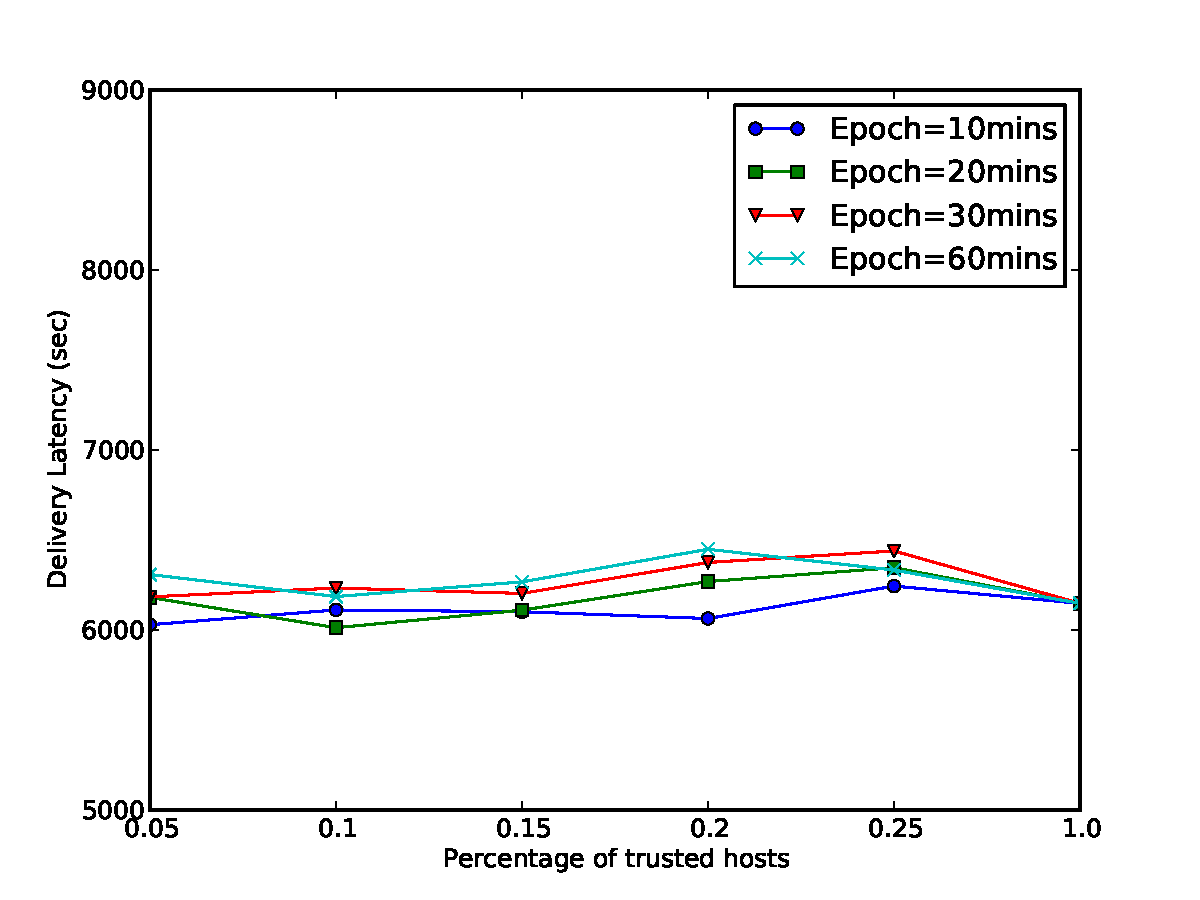
\includegraphics[width=0.49\columnwidth]{figures/epoch_3_overall/delivery_latency.pdf}
\label{fig:delivery_latency_3_overall}
}
\hfill
\subfloat[Ephemeral ID valid for 6 epochs]{%
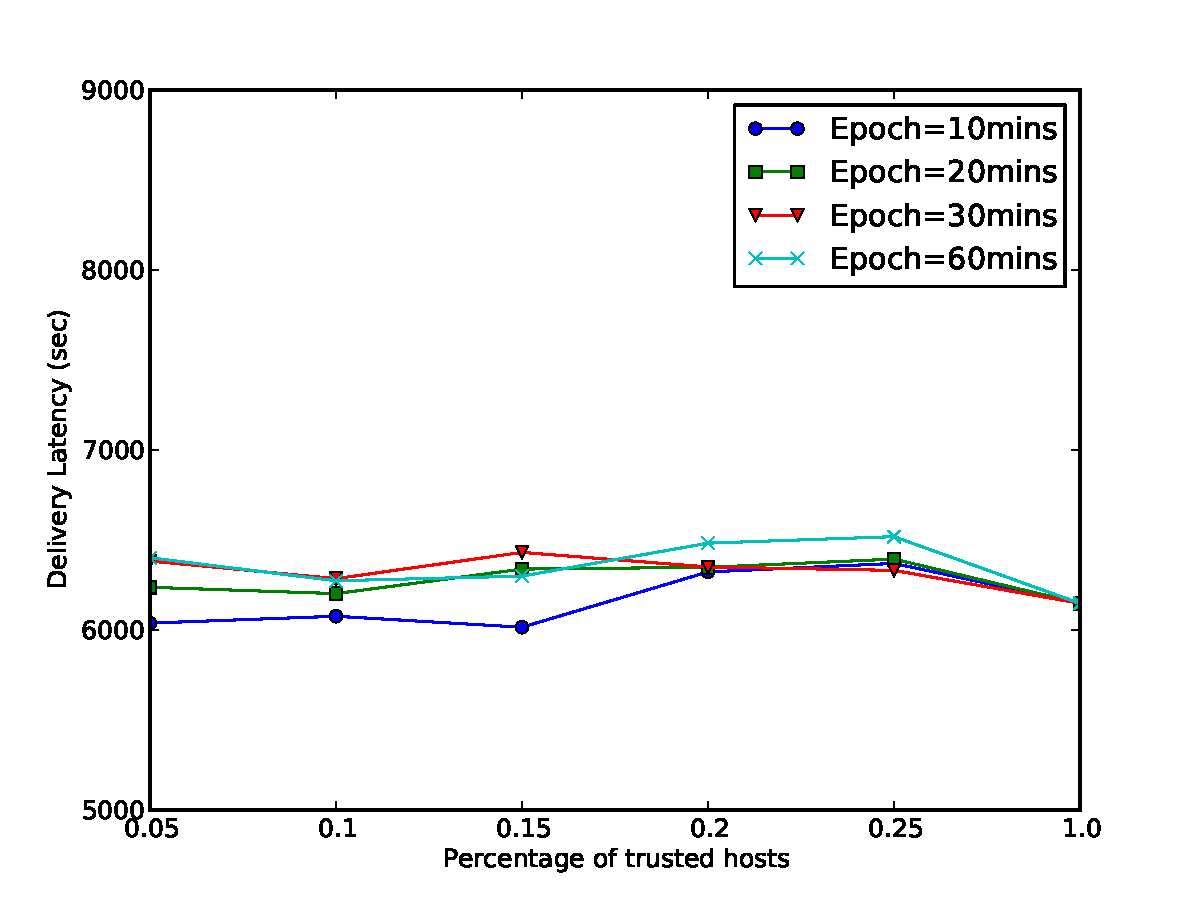
\includegraphics[width=0.49\columnwidth]{figures/epoch_6_overall/delivery_latency.pdf}
\label{fig:delivery_latency_6_overall}
}

\caption{{\bf Overall packet delivery latency.}
Overall packet delivery rate is almost same to that of epidemic routing. 
}
\label{fig:delivery_latency_overall}
\end{figure}




% hop count
\begin{figure}[h!]
\center
\subfloat[Ephemeral ID valid for 3 epochs]{%
\includegraphics[width=0.49\columnwidth]{figures/epoch_3_overall/hopcount.pdf}
\label{fig:delivery_hopcount_3_overall}
}
\hfill
\subfloat[Ephemeral ID valid for 6 epochs]{%
\includegraphics[width=0.49\columnwidth]{figures/epoch_6_overall/hopcount.pdf}
\label{fig:delivery_hopcount_6_overall}
}

\caption{{\bf Overall packet delivery hop count.}
Overall delivery hop count is almost same to that of epidemic routing. 
}
\label{fig:delivery_hopcount_overall}
\end{figure}



\end{document}







